\documentclass[preprint,12pt]{elsarticle}

\usepackage[T1]{fontenc}
\usepackage{microtype}
\usepackage{amsmath,amssymb,mathtools}
\usepackage{amsthm}
\usepackage{booktabs,tabularx,multirow,array,longtable}
\usepackage{graphicx}
\usepackage{xcolor}
\usepackage{enumitem}
\usepackage{hyperref}
\hypersetup{hidelinks}
\usepackage{lineno}
\usepackage{siunitx}
\usepackage{placeins}

\journal{Information Systems}

\newcommand{\ALG}{\operatorname{ALG}}
\newcommand{\Cov}{\operatorname{Cov}}
\newcommand{\R}{\mathbb{R}}
\newcommand{\ind}{\mathbf{1}}
\newcommand{\scos}{s_{\mathrm{cos}}}
\newcommand{\deltacos}{\delta_{\mathrm{cos}}}
\newcommand{\eps}{\varepsilon}
\newtheorem{proposition}{Proposition}

\begin{document}
\begin{frontmatter}

\title{Adaptive Local-Global Similarity for Comparing Heterogeneous Unordered Embedding Sets}

\author[talan,irit]{Nour Elhouda Kired\corref{cor1}}
\ead{nour.kired@talan.com}
\author[irit]{Olivier Teste}
\ead{olivier.teste@irit.fr}
\cortext[cor1]{Corresponding author.}
\address[talan]{Talan, Paris, France}
\address[irit]{IRIT, Universit\'e Toulouse-Jean Jaur\`es, Toulouse, France}

\begin{abstract}
Many information-system and machine-learning tasks compare finite unordered
sets of embeddings rather than individual vectors. Existing similarity measures
often emphasize either local neighborhood structure or global distributional
structure, although the two properties are complementary. We define Adaptive
Local-Global similarity (ALG), a symmetric similarity measure that combines a
local similarity with a global similarity. The local and global similarities and the resulting configurable ALG
similarity take values in $[0,1]$; the additive Initial ALG reference
instance is not constrained to this interval. The
local similarity uses adaptive $k$-nearest-neighbor scales, while the global
similarity is obtained by normalizing a distributional discrepancy. We evaluate ALG on 243 benchmark datasets from seven dataset families
(graphs, images, OpenML, tabular data, text, time series, and neural-model
activations).
The 243-dataset benchmark is divided into 60 training datasets and 186
held-out test datasets. A single configuration is selected on the 60
training datasets and then fixed before evaluation on the 186 held-out
test datasets. The selected configuration
reaches a mean positive-label F1-score across datasets of 0.7556, compared
with 0.7498 for Energy
distance, the strongest literature baseline with complete test coverage.
Ablation and controlled perturbation experiments further characterize the
complementarity of the local and global similarities and their response to
controlled distributional changes. These results support local-global
similarity as a reliable approach for comparing heterogeneous embedding sets.
\end{abstract}

\begin{keyword}
embedding-set similarity \sep adaptive neighborhoods \sep local similarity \sep
global similarity \sep distribution comparison
\end{keyword}

\end{frontmatter}

\linenumbers

\section{Introduction}
\label{sec:introduction}

Many data-integration and machine-learning pipelines represent an object by a
finite set of vectors. A database attribute can be represented by embeddings of
its name and values, a graph by node embeddings, an image by local descriptors,
a text by token or sentence embeddings, and a time series by embeddings of
sliding windows. Neural-network layers can also be represented by sets of hidden
activations. In these settings, the comparison problem is not the comparison of
two individual vectors, but the comparison of two finite unordered embedding
sets.

A similarity measure between embedding sets must account for more than one
property of the representation. Neighborhood-based measures describe local
support and density, but they can remain high when two embedding sets undergo a
coherent displacement. Global measures describe aggregate or distributional
differences, but a global summary can assign similar values to embedding sets
with different local structure. Kernel two-sample measures such as MMD compare
empirical distributions through a reproducing-kernel Hilbert space
\cite{gretton2012mmd}; optimal-transport measures compare the mass displacement
required to transform one empirical distribution into another
\cite{cuturi2013sinkhorn}; and nearest-neighbor measures estimate local support
from within-set neighborhoods
\cite{kynkaanniemi2019precision,naeem2020reliable,cheema2023prc}. These measures
capture different properties of the same embedding sets.

Figure~\ref{fig:motivation} illustrates the resulting limitation. Two embedding
sets can have similar global summaries while having different local support. In
the opposite case, two embedding sets can preserve similar local neighborhoods
while being globally displaced. A similarity measure based only on one of these
properties can therefore miss a difference that is explicit in the other.

\begin{figure*}[t]
\centering
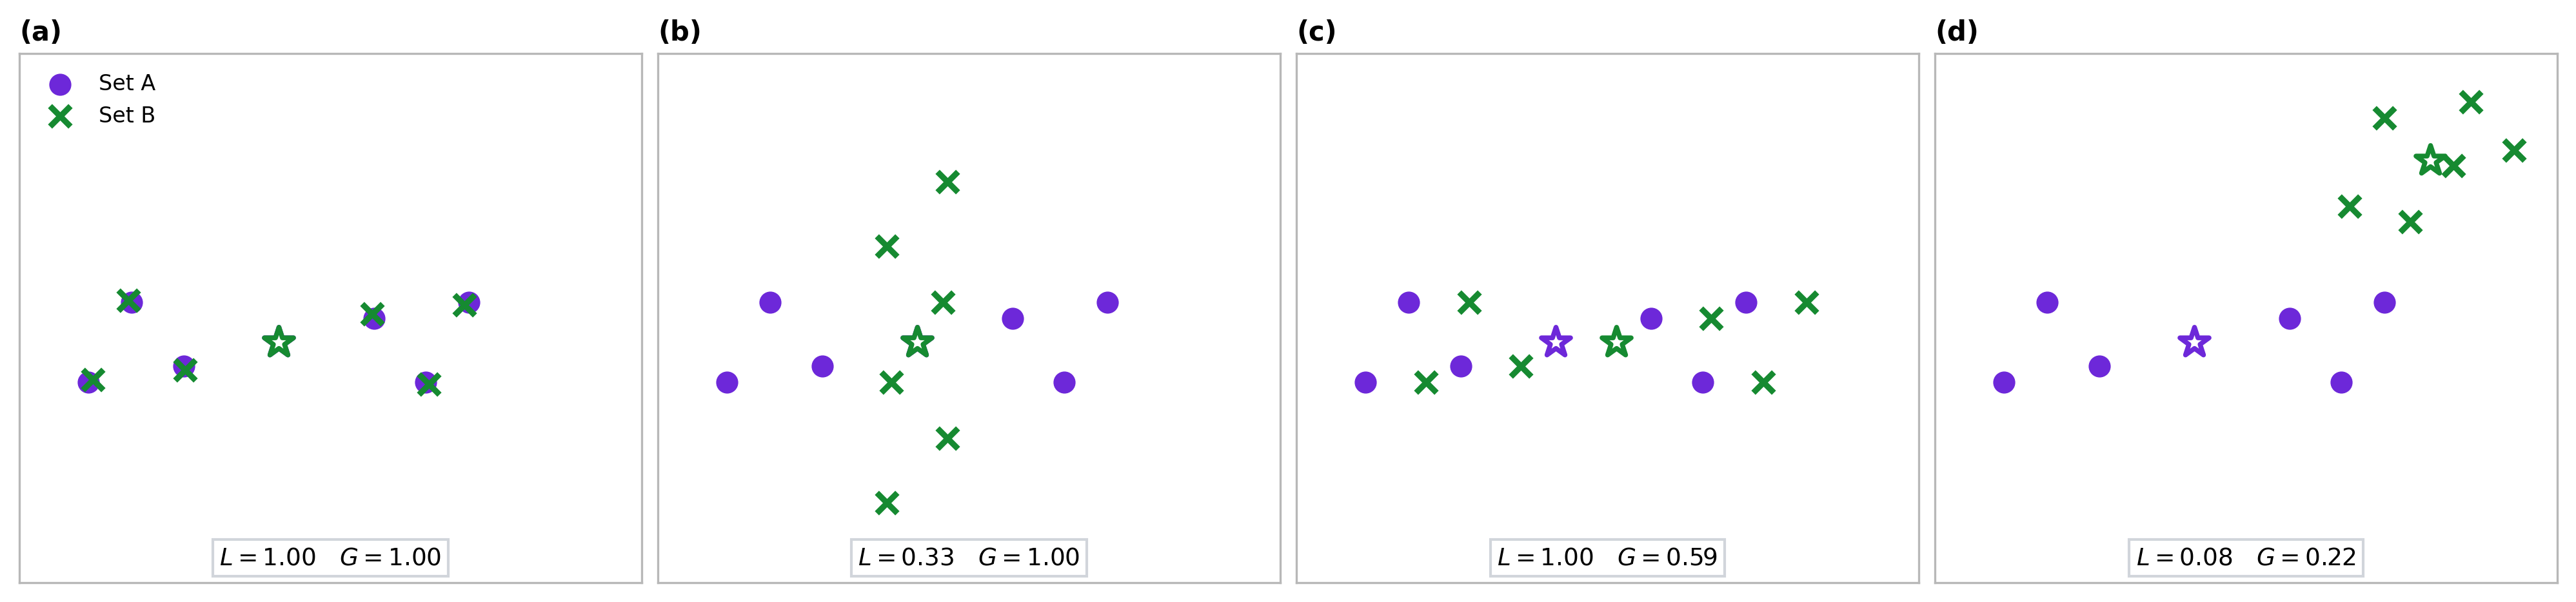
\includegraphics[width=0.96\textwidth]{figures/alg_local_global_motivation.png}
\caption{Local and global similarity capture complementary properties of two
embedding sets. A global summary can remain similar when local support changes,
whereas a local neighborhood similarity can remain high after a coherent global
displacement. ALG combines the two similarities explicitly.}
\label{fig:motivation}
\end{figure*}

The same issue is central to the evaluation of generative models and point-set
representations. Kynk\"a\"anniemi et al.~\cite{kynkaanniemi2019precision} use
sample-dependent nearest-neighbor radii to estimate local support. Naeem et
al.~\cite{naeem2020reliable} define Density and Coverage after identifying
failure cases of earlier precision-recall estimators. Cheema and
Urner~\cite{cheema2023prc} formalize bidirectional nearest-neighbor coverage,
while Khayatkhoei and AbdAlmageed~\cite{khayatkhoei2023asymmetry} show that
nearest-neighbor precision and recall can become asymmetric in high dimension.
For point sets, Chamfer distance, Earth Mover's Distance, and Density-Aware
Chamfer Distance retain different geometric information
\cite{fan2017pointsets,wu2021dcd}. These results motivate a similarity measure
in which local neighborhood structure and global distributional difference are
both explicit.

We first instantiate this idea as \emph{Initial ALG}: symmetric cosine
neighborhood coverage with $k=1$ plus cosine similarity between pooled
centroids. Initial ALG exposes the local-global principle but fixes the local
similarity, global similarity, geometry, and combination rule. We therefore
define \emph{Adaptive Local-Global similarity} (ALG) as the general configurable
formulation. The configuration selected only on the training datasets and then
frozen is denoted ALG$^*$.

The empirical evaluation separates configuration selection from final
evaluation. Configuration selection is performed on 60 training datasets,
one ALG configuration is selected, and that configuration is then fixed for
evaluation on 186 held-out test datasets. The evaluation covers 243
benchmark datasets and a search space of 168,960 ALG configurations; the frozen
configuration is also evaluated on three additional neural-model-activation
datasets.
The evaluation compares ALG with 38 literature baselines and two standard pooled
baselines, while internal ALG components are reported separately in ablation
analyses. 

\noindent  The contributions of this work are the following:
\begin{itemize}

    \item We define Initial ALG as the reference local-global instance and
    generalize it into ALG, a symmetric and permutation-invariant formulation
    for finite unordered embedding sets. ALG combines a candidate local
    similarity with a normalized candidate global similarity in a common
    range.

    \item We establish a unified configuration-selection and evaluation
    protocol across seven heterogeneous dataset families. The held-out test
    evaluation spans seven of these families. Our
    benchmark brings together 38 literature baselines
    from different research domains, including methods specifically
    designed for particular data families, alongside general-purpose
    similarity measures. ALG and all tunable baselines are configured
    exclusively on the same 60 training datasets, with their
    selected configurations fixed before evaluation on the same
    186 held-out test datasets in the completed evaluation. This protocol
    enables a consistent
    comparison of domain-specific and general-purpose methods across
    the evaluated dataset families, without dataset-specific or test-time
    configuration selection.

    \item We provide a large-scale empirical analysis of local-global
    similarity across heterogeneous embedding sets. The evaluation includes
    literature and pooled baselines, matched local-only and global-only
    ablations, cross-family analysis, controlled perturbation experiments,
    and computational-efficiency measurements. These experiments characterize
    when local and global similarities are complementary and how the compared
    similarity measures respond to controlled distributional changes.

\end{itemize}

The remainder of the paper is organized as follows.
Section~\ref{sec:related} reviews neighborhood-based, distributional, and
point-set similarity measures. Section~\ref{sec:method} defines ALG.
Section~\ref{sec:protocol} describes the experimental methodology.
Section~\ref{sec:results} reports and discusses the results, and
Section~\ref{sec:conclusion} concludes the paper.

\section{Related work}
\label{sec:related}

\subsection{Neighborhood-based similarity}

Nearest-neighbor methods estimate local properties directly from empirical
samples. Kynk\"a\"anniemi et al.~\cite{kynkaanniemi2019precision} represent an
empirical distribution by the union of hyperspheres centered on the observed
samples. The radius of each hypersphere is determined by a within-sample
$k$-nearest-neighbor distance, so the neighborhood scale changes with local
density. Precision and recall are then obtained by testing whether samples from
one distribution fall inside the empirical support of the other.

Naeem et al.~\cite{naeem2020reliable} analyze failure cases of these estimators
and define Density and Coverage to improve their reliability under outliers and
changes in neighborhood structure. Cheema and Urner~\cite{cheema2023prc} define
Precision Recall Cover using bidirectional nearest-neighbor relations and study
its mathematical properties. Khayatkhoei and
AbdAlmageed~\cite{khayatkhoei2023asymmetry} show that nearest-neighbor precision
and recall can exhibit systematic asymmetry as dimension increases. These works
establish both the usefulness and the limitations of adaptive local support.
ALG uses the same general principle for its local similarity: the scale of a
cross-set comparison is defined from within-set neighborhoods and the local
similarity is symmetrized.

\subsection{Global distributional similarity}

Global two-sample measures compare empirical distributions without reducing the
comparison to nearest-neighbor coverage. Maximum Mean Discrepancy (MMD) compares
distributions through differences in expectations over a reproducing-kernel
Hilbert space~\cite{gretton2012mmd,sriperumbudur2010embeddings}. Its empirical
behavior depends on the kernel and its bandwidth. Energy distance provides a
distance between distributions through expected pairwise distances, while
Fr\'echet-type measures summarize empirical distributions by low-order moments.
These measures capture global distributional differences but do not preserve
the same local neighborhood information as nearest-neighbor measures.

Optimal transport compares two empirical distributions through the cost of
transporting mass between them. Exact transport is computationally expensive;
entropic regularization and the Sinkhorn algorithm provide a practical
approximation~\cite{cuturi2013sinkhorn}, and sliced Wasserstein measures reduce
the computational burden through one-dimensional projections. In ALG, MMD,
Energy distance, Fr\'echet distance, centroid distance, and sliced Wasserstein
distance are treated as candidate global discrepancies that are normalized to a
common similarity range before being combined with the local similarity.

\subsection{Point-set distances}

Point-set distances provide another family of comparisons between finite sets.
Chamfer distance aggregates nearest-neighbor distances in both directions, but
many-to-one assignments can make it insensitive to density differences. Earth
Mover's Distance uses a global assignment and therefore retains different
information from Chamfer distance. Density-Aware Chamfer Distance (DCD) adds a
density correction to the nearest-neighbor comparison and bounds the resulting
measure~\cite{wu2021dcd}. The ALG configuration space includes a DCD-inspired
local similarity together with coverage, manifold precision-recall F1, best
buddies, and local scaling.

\subsection{Embedding-set comparison}

Data integration systems often rely on multiple similarity signals to handle
heterogeneous schemas and data representations. Classical schema matching
systems such as Cupid, COMA, and Similarity Flooding combine lexical,
instance-level, and structural evidence
\cite{madhavan2001cupid,do2002coma,melnik2002similarity}. More recent
embedding-based approaches improve the semantic representation of schema
elements and data values
\cite{koutras2021valentine,du2024isresmat,zhang2025smutf,liu2025magneto}.
Across these systems, combining complementary sources of information is
typically more effective than relying on a single signal, because different
signals capture different aspects of heterogeneity.

This observation also applies once objects are represented as sets of
embeddings. A remaining question is how two such sets should be compared
without collapsing their structure into a single representation or relying on
only one geometric criterion. ALG follows the same principle of complementary
evidence by combining local neighborhood information with global
distributional information in a single similarity measure.


\section{Adaptive Local-Global similarity}
\label{sec:method}

\subsection{Problem formulation}

Let
\[
    A=\{a_i\}_{i=1}^{n},
    \qquad
    B=\{b_j\}_{j=1}^{m},
    \qquad
    a_i,b_j\in\R^D,
\]
be two finite unordered embedding sets, with $n,m\geq2$.

Our objective is to compare $A$ and $B$ using two complementary sources of
information: their local neighborhood structure and their global
distributional structure. Since the embeddings are unordered, the similarity
must be permutation invariant. Moreover, because neither set is treated as a
reference, the similarity must be symmetric.

We first introduce the initial formulation that motivated ALG. We then
generalize this formulation by allowing the local similarity, the global
similarity, their underlying geometries, and their relative contributions to
vary.

% -
\subsection{Initial ALG}

Initial ALG combines a local similarity based on bidirectional neighborhood
coverage with a global similarity based on the cosine similarity between the
two set centroids.

\paragraph{Local similarity.}

Let $d$ be a non-negative dissimilarity. For each $a_i\in A$, we define its
within-set $k$-nearest-neighbor radius as
\begin{equation}
\rho_A^{(k)}(a_i)
=
d\!\left(
a_i,
\operatorname{kNN}_k(a_i;A\setminus\{a_i\})
\right),
\label{eq:radius}
\end{equation}
and define $\rho_B^{(k)}$ analogously.

The directed coverage from $A$ to $B$ is the proportion of points in $A$
whose nearest point in $B$ lies within their within-set neighborhood radius:
\begin{equation}
\Cov_d^{(k)}(A\!\to\!B)
=
\frac{1}{n}
\sum_{i=1}^{n}
\ind\!\left[
\min_{b\in B}d(a_i,b)
\leq
\rho_A^{(k)}(a_i)
\right].
\label{eq:directed-coverage}
\end{equation}

The same quantity is computed from $B$ to $A$, and the two directions are
averaged to obtain the symmetric coverage similarity:
\begin{equation}
L_{\mathrm{cov},d}^{(k)}(A,B)
=
\frac{1}{2}
\left[
\Cov_d^{(k)}(A\!\to\!B)
+
\Cov_d^{(k)}(B\!\to\!A)
\right].
\label{eq:coverage}
\end{equation}

The neighborhood radius is estimated from each embedding set itself and
therefore adapts to local density. This principle is related to empirical
precision, recall, density, and coverage measures
\cite{kynkaanniemi2019precision,naeem2020reliable,cheema2023prc}.

Initial ALG uses $k=1$ and cosine dissimilarity. For nonzero vectors $x$ and
$y$, cosine dissimilarity is defined as
\begin{equation}
\deltacos(x,y)
=
1-
\frac{x^\top y}
{\lVert x\rVert_2\lVert y\rVert_2}.
\label{eq:cosine-dissimilarity}
\end{equation}

Thus, the local similarity measures the proportion of points from each set
that are covered by the other set relative to the local neighborhood scale of
the original set.

\paragraph{Global similarity.}

The global similarity first summarizes each embedding set by its centroid:
\begin{equation}
\mu_A
=
\frac{1}{n}\sum_{i=1}^{n}a_i,
\qquad
\mu_B
=
\frac{1}{m}\sum_{j=1}^{m}b_j.
\label{eq:centroids}
\end{equation}

The global similarity is then defined as the cosine similarity between these
two centroids:
\begin{equation}
S_{\mathrm{cos}}^{\mathrm{cent}}(A,B)
=
\frac{\mu_A^\top\mu_B}
{\lVert\mu_A\rVert_2\lVert\mu_B\rVert_2}.
\label{eq:centroid-cosine}
\end{equation}

Initial ALG combines the local and global similarities as
\begin{equation}
\ALG_{\mathrm{init}}(A,B)
=
L_{\mathrm{cov},\deltacos}^{(1)}(A,B)
+
S_{\mathrm{cos}}^{\mathrm{cent}}(A,B).
\label{eq:initial-alg}
\end{equation}

This initial formulation captures the central intuition of ALG: two embedding
sets should be compared using both local and global information. However, it
fixes one particular local similarity, one particular global similarity, and
a fixed combination of the two. Moreover, because centroid cosine similarity
takes values in $[-1,1]$, Initial ALG is not constrained to $[0,1]$.

We therefore generalize this formulation into a bounded and configurable
local-global similarity.

% -
\subsection{ALG formulation}

Let
\[
0\leq L(A,B)\leq1
\qquad\text{and}\qquad
0\leq G(A,B)\leq1
\]
denote a bounded local similarity and a bounded global similarity,
respectively.

ALG is defined as
\begin{equation}
\ALG_{L,G,\lambda}(A,B)
=
\lambda L(A,B)
+
(1-\lambda)G(A,B),
\qquad
\lambda\in[0,1].
\label{eq:alg}
\end{equation}

We refer to $\lambda$ as the \emph{local-global weight}. It controls the
relative contribution of the two similarities. The endpoints $\lambda=1$
and $\lambda=0$ correspond respectively to local-only and global-only
similarities, whereas intermediate values combine both sources of
information.

\begin{proposition}[Structural properties]
Suppose that $L$ and $G$ are symmetric, permutation invariant, and bounded
in $[0,1]$. Then, for every $\lambda\in[0,1]$,
$\ALG_{L,G,\lambda}$ is symmetric, permutation invariant, and bounded
in $[0,1]$.
\end{proposition}

\begin{proof}
Symmetry and permutation invariance are preserved by scalar multiplication and
addition. Boundedness follows because Eq.~\eqref{eq:alg} is a convex
combination of two values in $[0,1]$.
\end{proof}

Rather than fixing $L$ and $G$ a priori, we evaluate several candidate local
and global similarities and select their configuration using only the
training datasets.

% -
\subsection{Candidate local similarities}

The local similarity captures how similarly the two embedding sets are
organized at the neighborhood level.

For neighborhood-based similarities, the radius defined in
Eq.~\eqref{eq:radius} provides an adaptive local scale. It is smaller in dense
regions and larger in sparse regions, allowing distances between the two sets
to be interpreted relative to their local neighborhood structure.

Coverage, defined in Eq.~\eqref{eq:coverage}, is the local similarity used in
Initial ALG. ALG also considers alternative local similarities.

One such candidate is the \emph{local-scaling similarity}. Let
\[
j(i)=\arg\min_j d(a_i,b_j)
\]
denote the nearest point in $B$ to $a_i$, and define $i(j)$ analogously for
the reverse direction. The directed local-scaling similarity from $A$ to $B$
is
\begin{equation}
L_{A\to B,d}^{(k)}
=
\frac{1}{n}
\sum_{i=1}^{n}
\exp\!\left(
-\frac{
d(a_i,b_{j(i)})^2
}{
\rho_A^{(k)}(a_i)
\rho_B^{(k)}(b_{j(i)})
}
\right).
\label{eq:local-directed}
\end{equation}

The symmetric local-scaling similarity is
\begin{equation}
L_{\mathrm{LS},d}^{(k)}(A,B)
=
\frac{1}{2}
\left(
L_{A\to B,d}^{(k)}
+
L_{B\to A,d}^{(k)}
\right).
\label{eq:local-scaling}
\end{equation}

The denominator normalizes the distance between matched points using their
within-set neighborhood scales. Consequently, the same absolute displacement
receives a larger penalty in a dense region than in a sparse region. This
construction is related to self-tuning neighborhood kernels
\cite{zelnikmanor2004selftuning}.

The \emph{Manifold PR-F1} candidate uses the same within-set radii to form two
empirical manifolds. Its precision and recall are
\begin{align}
P_d^{(k)}(A,B)
&=\frac{1}{m}\sum_{j=1}^{m}
\ind\!\left[\exists i:\ d(a_i,b_j)\leq\rho_A^{(k)}(a_i)\right],\\
R_d^{(k)}(A,B)
&=\frac{1}{n}\sum_{i=1}^{n}
\ind\!\left[\exists j:\ d(a_i,b_j)\leq\rho_B^{(k)}(b_j)\right].
\end{align}
The local similarity is their harmonic mean,
$L_{\mathrm{MPR},d}^{(k)}=2PR/(P+R)$, with value zero when $P+R=0$.

For \emph{Best Buddies}, let $j(i)$ be the nearest point in $B$ to $a_i$ and
$i(j)$ the nearest point in $A$ to $b_j$. The similarity is the fraction of
mutual nearest-neighbor pairs normalized by the smaller set:
\begin{equation}
L_{\mathrm{BB},d}(A,B)=
\frac{1}{\min(n,m)}\sum_{i=1}^{n}\ind[i(j(i))=i].
\end{equation}

The \emph{DCD-inspired} candidate additionally penalizes many-to-one nearest
neighbor assignments. Define
$c_B(j)=\max\{1,\sum_i\ind[j(i)=j]\}$ and
$c_A(i)=\max\{1,\sum_j\ind[i(j)=i]\}$. For $\alpha>0$,
\begin{equation}
L_{\mathrm{DCD},d}^{(\alpha)}(A,B)=\frac{1}{2}
\left[
\frac{1}{n}\sum_i\frac{e^{-\alpha d(a_i,b_{j(i)})^2}}{c_B(j(i))}
+
\frac{1}{m}\sum_j\frac{e^{-\alpha d(a_{i(j)},b_j)^2}}{c_A(i(j))}
\right].
\end{equation}

The complete search space contains five local-similarity families and four
base dissimilarities: Euclidean, Manhattan, Chebyshev, and cosine
dissimilarity.

\begin{table}[!htbp]
\centering
\caption{Local-similarity search space.}
\label{tab:local-search-space}
\small
\begin{tabularx}{\linewidth}{lXr}
\toprule
Local similarity & Parameters & Count\\
\midrule
Coverage
& 4 dissimilarities $\times\ k\in\{1,3,5,10\}$
& 16\\
Local scaling
& 4 dissimilarities $\times\ k\in\{1,3,5,10\}$
& 16\\
Manifold PR-F1
& 4 dissimilarities $\times\ k\in\{1,3,5,10\}$
& 16\\
DCD-inspired
& 4 dissimilarities $\times\ \alpha\in\{10,50,100\}$
& 12\\
Best Buddies
& 4 dissimilarities
& 4\\
\midrule
Total & & 64\\
\bottomrule
\end{tabularx}
\end{table}

The neighborhood parameter $k$ is included whenever the corresponding local
similarity depends on a neighborhood radius.

% -
\subsection{Candidate global similarities}

The global similarity is obtained from a \emph{global discrepancy}. We define
a global discrepancy $\Delta_g(A,B)\geq0$ as a non-negative quantity measuring
the overall difference between the two embedding sets according to a chosen
distributional or geometric criterion. Because a global discrepancy increases
as the two sets become less similar, it must be transformed before being
combined with the local similarity.

We consider eight global discrepancies. Four compare the centroids
$\mu_A$ and $\mu_B$ using Euclidean, Manhattan, Chebyshev, or cosine
dissimilarity. The remaining global discrepancies are Energy distance,
RBF-MMD, Gaussian Fr\'echet distance, and sliced Wasserstein distance.

\begin{table}[!htbp]
\centering
\caption{Global-discrepancy search space before normalization.}
\label{tab:global-search-space}
\small
\begin{tabularx}{\linewidth}{lXr}
\toprule
Global discrepancy & Geometry or specification & Count\\
\midrule
Centroid
& Euclidean, Manhattan, Chebyshev, cosine dissimilarity
& 4\\
Energy
& Euclidean pairwise geometry
& 1\\
RBF-MMD
& RBF kernel with median-bandwidth rule
& 1\\
Gaussian Fr\'echet
& Mean and covariance discrepancy
& 1\\
Sliced Wasserstein
& Euclidean projected transport
& 1\\
\midrule
Total & & 8\\
\bottomrule
\end{tabularx}
\end{table}

The global discrepancies have different numerical ranges and therefore cannot
be directly combined with the local similarities. Each global
discrepancy $\Delta_g(A,B)$ is transformed into a global similarity:
\begin{equation}
G_{g,\psi,s}(A,B)
=
\psi\!\left(
\frac{
\Delta_g(A,B)
}{
s\,\sigma_g(A,B)
}
\right),
\label{eq:global}
\end{equation}
where $\sigma_g(A,B)>0$ is a reference scale, $s>0$ is a scale multiplier,
and
\[
\psi:[0,\infty)\rightarrow[0,1]
\]
is a monotonically decreasing normalization function.

We evaluate six normalization families. The clipped linear normalization is
geometry-specific:
\begin{align}
\psi_{\mathrm{lin},\cos}(z)&=\max(0,1-z/2),\\
\psi_{\mathrm{lin},d}(z)&=\max(0,1-z),
\quad d\in\{L_2,L_1,L_\infty\}.
\end{align}
The remaining five normalization functions are
\[
\frac{1}{1+z},\qquad
\frac{1}{1+z^2},\qquad
e^{-z},\qquad
e^{-z^2/2},\qquad
\frac{2}{1+e^z},
\]
corresponding respectively to rational, Cauchy, exponential, Gaussian, and
logistic normalization.

Each normalization is evaluated with
\[
s\in\{0.25,0.5,1,2,4\}.
\]

Consequently, each global discrepancy produces
\[
6\times5=30
\]
normalized global similarities. With eight global discrepancies, this gives
\[
8\times30=240
\]
candidate global similarities.

For centroid-based global discrepancies,
\begin{equation}
\Delta_{\mathrm{cent},d}(A,B)
=
d(\mu_A,\mu_B).
\label{eq:centroid-global}
\end{equation}

For cosine centroid discrepancy,
\[
\Delta_{\mathrm{cent},\cos}(A,B)
=
\deltacos(\mu_A,\mu_B),
\]
with $\sigma_g=1$.

Let $r(A,B)$ denote the median of the pooled within-set one-nearest-neighbor
distances in $A$ and $B$, lower-bounded by machine precision. The reference
scale is $\sigma_g=r(A,B)$ for centroid Euclidean, Manhattan, and Chebyshev
discrepancies, Energy distance, and sliced Wasserstein distance;
$\sigma_g=1$ for centroid cosine discrepancy and RBF-MMD; and
$\sigma_g=r(A,B)^2$ for Gaussian Fr\'echet distance. Sliced Wasserstein uses
32 unit-normalized Gaussian projection directions generated with random seed
zero. For every neighborhood-based local similarity, the effective value is
$\min(k,n-1)$ within a set of size $n$. Cosine distances involving a zero
vector are assigned the neutral dissimilarity value one, and denominators are
lower-bounded by machine precision.

% -
\subsection{Configuration space and selection}

ALG jointly varies the local similarity, the global similarity, and the
local-global weight.

The search space contains
\begin{itemize}
    \item 64 local similarities;
    \item 240 global similarities;
    \item 11 local-global weights,
    $\lambda\in\{0,0.1,\ldots,1\}$.
\end{itemize}

The complete search space therefore contains
\begin{equation}
64\times240\times11
=
168{,}960
\label{eq:configuration-space}
\end{equation}
ALG configurations.

All configuration choices are made exclusively on the training datasets,
as described in Section~\ref{sec:protocol}. The selected configuration is
then fixed before evaluation on the held-out test datasets. The configuration
selected by this procedure is reported in Section~\ref{sec:results} together
with its empirical evaluation.

% -
\subsection{Computational complexity}

With dense pairwise computations, estimating the within-set neighborhood
radii and cross-set nearest neighbors requires
\[
O\!\left((n^2+m^2+nm)D\right)
\]
operations.

The complete configuration space does not require the pairwise
dissimilarities to be recomputed for every ALG configuration. Pairwise
dissimilarity matrices are computed once and reused to evaluate the candidate
local similarities and global similarities. The local-global weight is then
applied without recomputing the pairwise dissimilarities.

This factorization makes configuration selection computationally feasible.

\section{Experimental methodology}
\label{sec:protocol}

The experimental methodology separates configuration selection from final
evaluation. All choices that define ALG$^*$ are made using the training
datasets. The held-out test datasets are used only after the selected ALG
configuration has been fixed.

\subsection{Research questions}

The experimental evaluation addresses five research questions:

\begin{itemize}
    \item \textbf{RQ1 - Effectiveness:} How effectively do Initial ALG and
    training-selected ALG$^*$ distinguish similar from dissimilar embedding
    sets compared with the complete baseline suite, overall, across dataset
    families, and on neural-model activations?

    \item \textbf{RQ2 - Ablation:} For Initial ALG and ALG$^*$, what is the
    contribution of the local similarity, the global similarity, and their
    local-global combination?

    \item \textbf{RQ3 - Configuration Stability:} Is the configuration selected
    on the training datasets supported by stable training and held-out test
    rankings and by a broad near-optimal region?

    \item \textbf{RQ4 - Sensitivity:} How do ALG$^*$, Initial ALG, and the
    baseline measures respond to controlled changes in local and global
    structure?

    \item \textbf{RQ5 - Efficiency:} How computationally efficient is ALG
    compared with the baseline measures, and what is the one-time cost of
    configuration selection?
\end{itemize}

\subsection{Datasets}

The benchmark resolver contains 250 candidate datasets from seven
dataset families. Seven datasets are excluded before configuration selection:
one image dataset has an incomplete computation and six time-series datasets
contain a non-finite or unavailable ALG component. The benchmark
therefore contains 243 eligible datasets and 208,725 labeled embedding-set
pairs, split at the dataset level into 60 training datasets (53,332 pairs) and
186 held-out test datasets (155,393 pairs). No dataset appears in both
partitions.

\begin{table}[!htbp]
\centering
\caption{Dataset-level training/test split.}
\label{tab:partition}
\small
\begin{tabular}{lrr}
\toprule
Dataset family & Training & Test\\
\midrule
Graphs & 6 & 15\\
Images & 5 & 12\\
OpenML & 15 & 57\\
Tabular & 2 & 1\\
Text & 1 & 6\\
Time series & 30 & 92\\
Neural-model activations & 1 & 3\\
\midrule
Total & 60 & 186\\
\bottomrule
\end{tabular}
\end{table}

Each dataset is converted into labeled pairs of embedding sets according to its
native representation. Graph datasets use node and spectral descriptors; image
datasets use local patches; OpenML and tabular datasets use class-conditional
row or image-patch representations; text datasets use sentence or token
representations; and time-series datasets use sliding-window representations.
The neural-model-activation dataset uses sets of hidden activations and belongs
to the training partition. Each eligible
dataset contributes up to 1,000 labeled embedding-set pairs in total, balanced
between positive and negative pairs whenever possible, with smaller datasets
contributing all valid pairs. The released dataset catalog
records the source collection, source URL, construction rule, pair count,
eligibility decision, partition, and redistribution status for every candidate
dataset.

After configuration selection, the fixed ALG$^*$ configuration and the complete. For each source dataset, multilayer
perceptrons with four hidden-layer architectures and five random seeds are fit
on 5,000 samples from the official training split. Hidden activations are then
extracted from a disjoint 1,000-sample subset of the official test split. This
produces 20 activation-set representations and 80 labeled pairs per dataset.
These three datasets are not used for ALG configuration selection.

\subsection{Threshold calibration}

Each similarity measure produces a scalar value and requires a threshold for
binary evaluation. No downstream classifier is trained for these scalar
similarities; C2ST remains classifier-based by definition. Within each dataset, we use
stratified five-fold cross-validation. For each fold, the threshold that
maximizes the positive-label F1-score ($y=1$) is selected on the other four
folds and then applied without change to the held-out fold. The five held-out
prediction vectors are pooled, and one positive-label F1-score is computed as
\begin{equation}
F1_{y=1}=\frac{2TP}{2TP+FP+FN}.
\label{eq:positive-f1}
\end{equation}
This is equivalent to micro-F1 restricted to label 1; it is not macro-averaged
over labels 0 and 1. This protocol evaluates the discriminative
ordering induced by the similarity measure while avoiding threshold selection
on the evaluated fold.

Threshold calibration is distinct from configuration selection. For ALG,
all 168,960 configurations are ranked by the unweighted mean of their
positive-label F1-scores across the 60 training datasets. The highest-ranked
configuration is then fixed before evaluation on the 186 held-out test datasets.

For every tunable baseline, candidate configurations are evaluated on the
same 60 training datasets and selected by the same unweighted mean
positive-label F1-score criterion. The selected configuration of each baseline
is fixed before the held-out evaluation. Baselines without tunable
configurations retain their fixed definitions. No configuration is selected
separately for an individual dataset or dataset family, and no held-out test
dataset is used to select a configuration. The local similarity, global
discrepancy, geometry, normalization, scale multiplier, and local-global
weight of ALG$^*$ remain fixed throughout the held-out evaluation.

\subsection{Baselines and ALG variants}

We distinguish four roles. ALG denotes the configurable formulation. Initial
ALG denotes its reference instance, introduced to motivate the local-global
construction. ALG$^*$ denotes the single configuration selected on the training
datasets and frozen before held-out evaluation. Internal ALG components and
alternative ALG configurations are used only for ablation or configuration
analysis; they are not additional proposed methods. All remaining comparison
methods are baselines.

The baseline suite contains 38 literature baselines and two standard pooled
baselines. The literature baselines cover neighborhood-based measures,
precision-recall and Density/Coverage measures, point-set distances,
distribution distances, kernel two-sample measures, optimal-transport measures,
classifier two-sample tests, and geometric or topological measures. The two
standard pooled baselines are included explicitly because they provide the
simplest global comparison after mean pooling:
\begin{align}
S_{\mathrm{cos}}^{\mathrm{pool}}(A,B)
&= \scos(\mu_A,\mu_B),\\
S_{\mathrm{Euc}}^{\mathrm{pool}}(A,B)
&= -\lVert \mu_A-\mu_B\rVert_2.
\label{eq:pooled-baselines}
\end{align}
The negative sign in the Euclidean baseline only converts a distance into a
similarity so that larger values consistently indicate greater similarity.
These two baselines test whether comparing the mean embeddings alone is
sufficient.

Table~\ref{tab:baseline-taxonomy} separates methodological family from original
application domain. The distinction matters because the benchmark deliberately
places methods developed for generative-image evaluation, point-cloud
reconstruction, image matching, spectral clustering, and general statistical
two-sample comparison in the same heterogeneous evaluation. ``Domain-oriented''
describes the setting in which a method was introduced; it does not restrict
the datasets on which the method is evaluated here.

\begin{table*}[!htbp]
\centering
\caption{Organization of the 40 baselines by methodological family and original
application domain. Every baseline remains in the overall and cross-family
comparisons.}
\label{tab:baseline-taxonomy}
\small
\begin{tabularx}{\textwidth}{>{\raggedright\arraybackslash}p{0.20\textwidth}>{\raggedright\arraybackslash}X>{\raggedright\arraybackslash}p{0.20\textwidth}}
\toprule
Methodological family & Included baselines & Original application domain\\
\midrule
Distribution and kernel comparison & Energy distance, MMD-RBF, KID, Gaussian
Fr\'echet, C2ST & Statistical two-sample testing or generative-model evaluation\\
Optimal transport & Sliced Wasserstein, Earth Mover/Wasserstein, Sinkhorn
divergence, Gromov-Wasserstein & General distribution comparison and geometric matching\\
Adaptive neighborhoods & Local-scaling affinity & Spectral clustering\\
Fidelity and diversity & PRD F1-max, manifold precision/recall, PRDC variants,
Coverage, clipped Density/Coverage, Precision-Recall Cover, alpha precision,
beta recall, and authenticity & Generative-model evaluation\\
Point-set geometry & Chamfer, modified Hausdorff, Hausdorff-95, Hausdorff,
Density-Aware Chamfer, and point-cloud F-score & Image matching or 3D point-cloud reconstruction\\
Mutual-neighbor and topology & Best Buddies, persistence bottleneck, and
Geometry Score & Image matching or generative-model geometry\\
Pooled representation & Pooled cosine and Pooled Euclidean & General-purpose embedding comparison\\
\bottomrule
\end{tabularx}
\end{table*}

Pooled cosine has two roles in the analysis that refer to the same computed
similarity: it is a standard pooled baseline in the baseline comparison and it
is exactly the global-only component of Initial ALG in the matched ablation.
It is therefore not recomputed or treated as a different method in the
ablation. The local-only component of Initial ALG is the symmetric cosine
overlap with $k=1$ defined in Eq.~\eqref{eq:initial-alg}; it remains an
internal ALG component rather than a baseline. Pooled Euclidean is not a
component of Initial ALG and is included only as a standard pooled baseline.

The fixed method taxonomy therefore contains the Initial ALG reference instance,
ALG$^*$, 40 baseline outputs, and six internal ALG components or alternative
configurations.
In the completed campaign, 40 baselines, Initial ALG, and ALG$^*$ are available
on all 186 held-out test datasets. Gaussian Fr\'echet is available on 133 test
datasets and is never imputed. We report its coverage explicitly and retain a
separate 133-dataset common-subset analysis in the results. The supplied
136-dataset graphic additionally includes the three neural-model-activation
datasets and is not used to represent the 133-dataset confirmatory subset. No
baseline is removed on the basis of its observed F1-score.

\subsection{Statistical analysis}

The unit of statistical analysis is the dataset. Unless explicitly stated
otherwise, reported means are unweighted means of the per-dataset
positive-label F1-scores; they are not obtained by pooling predictions across
datasets. We report mean and median positive-label F1-score, fractional dataset
wins, strict and tied dataset wins, and paired wins/ties/losses. For each
ALG-versus-baseline comparison, the mean paired F1-score difference is
accompanied by a 95\% confidence interval estimated from 10,000 paired bootstrap
resamples. We also use the Wilcoxon signed-rank test and apply Holm correction
over the complete set of 40 baseline comparisons separately for Initial ALG
and ALG$^*$. Pairing is performed at the dataset level so that
differences in dataset difficulty do not confound the comparison.

The ranking of all configurations on the held-out test datasets is used only as
a post-hoc stability analysis. It is not used to redefine ALG$^*$ or to make a
second configuration selection.

\subsection{Controlled perturbation experiments}

The held-out benchmark measures discrimination on real datasets but does not
identify which distributional changes each similarity measure detects. We
therefore use controlled perturbation experiments following the diagnostic
logic of Naeem et al.~\cite{naeem2020reliable}. The full campaign contains 145
perturbation conditions and 128 random seeds, corresponding to 18,560
condition-seed evaluations. The conditions include translation, variance
change, outliers, cardinality imbalance, dimension, duplicates, nested and
non-convex supports, rings, collapsed arcs, filled disks, and sequential or
simultaneous mode removal. A dedicated protocol also evaluates Gaussian
mixtures, mean shifts, outliers, and mode removal.

The controlled perturbation experiments are not used for ALG configuration
selection. They are diagnostic experiments: as perturbation severity increases,
a similarity measure is expected to change monotonically when the perturbation
corresponds to information represented by that measure. Failure to respond is
therefore interpreted as an invariance or limitation of the underlying
geometry, not as a configuration-selection result.

\section{Results}
\label{sec:results}

We evaluate 168,960 ALG configurations on 243 benchmark datasets: 60 training
datasets and 186 held-out test datasets. The frozen configuration and the
baseline suite are additionally evaluated on three neural-model-activation
datasets.

\subsection{Selected ALG configuration}

Configuration selection is performed only on the 60 training datasets.
Among the configurations in the completed search campaign, the selected
configuration combines local scaling with Manhattan distance and $k=3$ with a
normalized cosine-centroid global similarity. Its local-global weight is
$\lambda=0.7$:
\begin{equation}
\boxed{
\ALG^*(A,B)=
0.7\,L_{\mathrm{LS},\,L_1,\,k=3}(A,B)
+
0.3\exp\!\left[
-\frac{\deltacos(\mu_A,\mu_B)}{2}
\right]
}
\label{eq:selected-alg}
\end{equation}

Thus, the selected configuration gives greater weight to the adaptive local
component while retaining a non-zero global contribution. This configuration
is fixed before evaluation on the 186 held-out test datasets.

\subsection{RQ1: Effectiveness}

Table~\ref{tab:main} reports the principal comparison on the 186 held-out
test datasets. Figure~\ref{fig:leaderboard} contains ALG$^*$,
Initial ALG, and the 40 baselines with complete test coverage, including
Pooled cosine and Pooled Euclidean. Internal ALG similarities are not included
in this comparison. The means in the figure and Table~\ref{tab:main} use
different dataset populations and should not be compared as identical estimates.

ALG$^*$ obtains the highest mean positive-label F1-score across datasets,
0.7556. Initial ALG
reaches 0.7507, and Energy distance, the strongest literature baseline with
complete test coverage, reaches 0.7498. The difference between ALG$^*$ and
Initial ALG is an internal comparison and measures the effect of configuration
selection within ALG. The baseline comparison evaluates ALG against the 38
literature baselines and the two standard pooled baselines. Pooled cosine and
Pooled Euclidean reach mean positive-label F1-scores of 0.7392 and 0.7386,
respectively.

\begin{table}[!htbp]
\centering
\caption{Summary of the held-out comparison. The complete baseline ranking is
reported in Figure~\ref{fig:leaderboard}.}
\label{tab:main}
\small
\begin{tabular}{lrrr}
\toprule
Method & $n$ & Mean $F1_{y=1}$ & Median $F1_{y=1}$\\
\midrule
ALG$^*$ & 186 & \textbf{0.7556} & \textbf{0.6871}\\
Initial ALG & 186 & \underline{0.7507} & 0.6813\\
Energy distance & 186 & 0.7498 & \underline{0.6852}\\
Pooled cosine & 186 & 0.7392 & 0.6698\\
Pooled Euclidean & 186 & 0.7386 & 0.6707\\
\bottomrule
\end{tabular}
\end{table}

\begin{figure*}[!htbp]
\centering
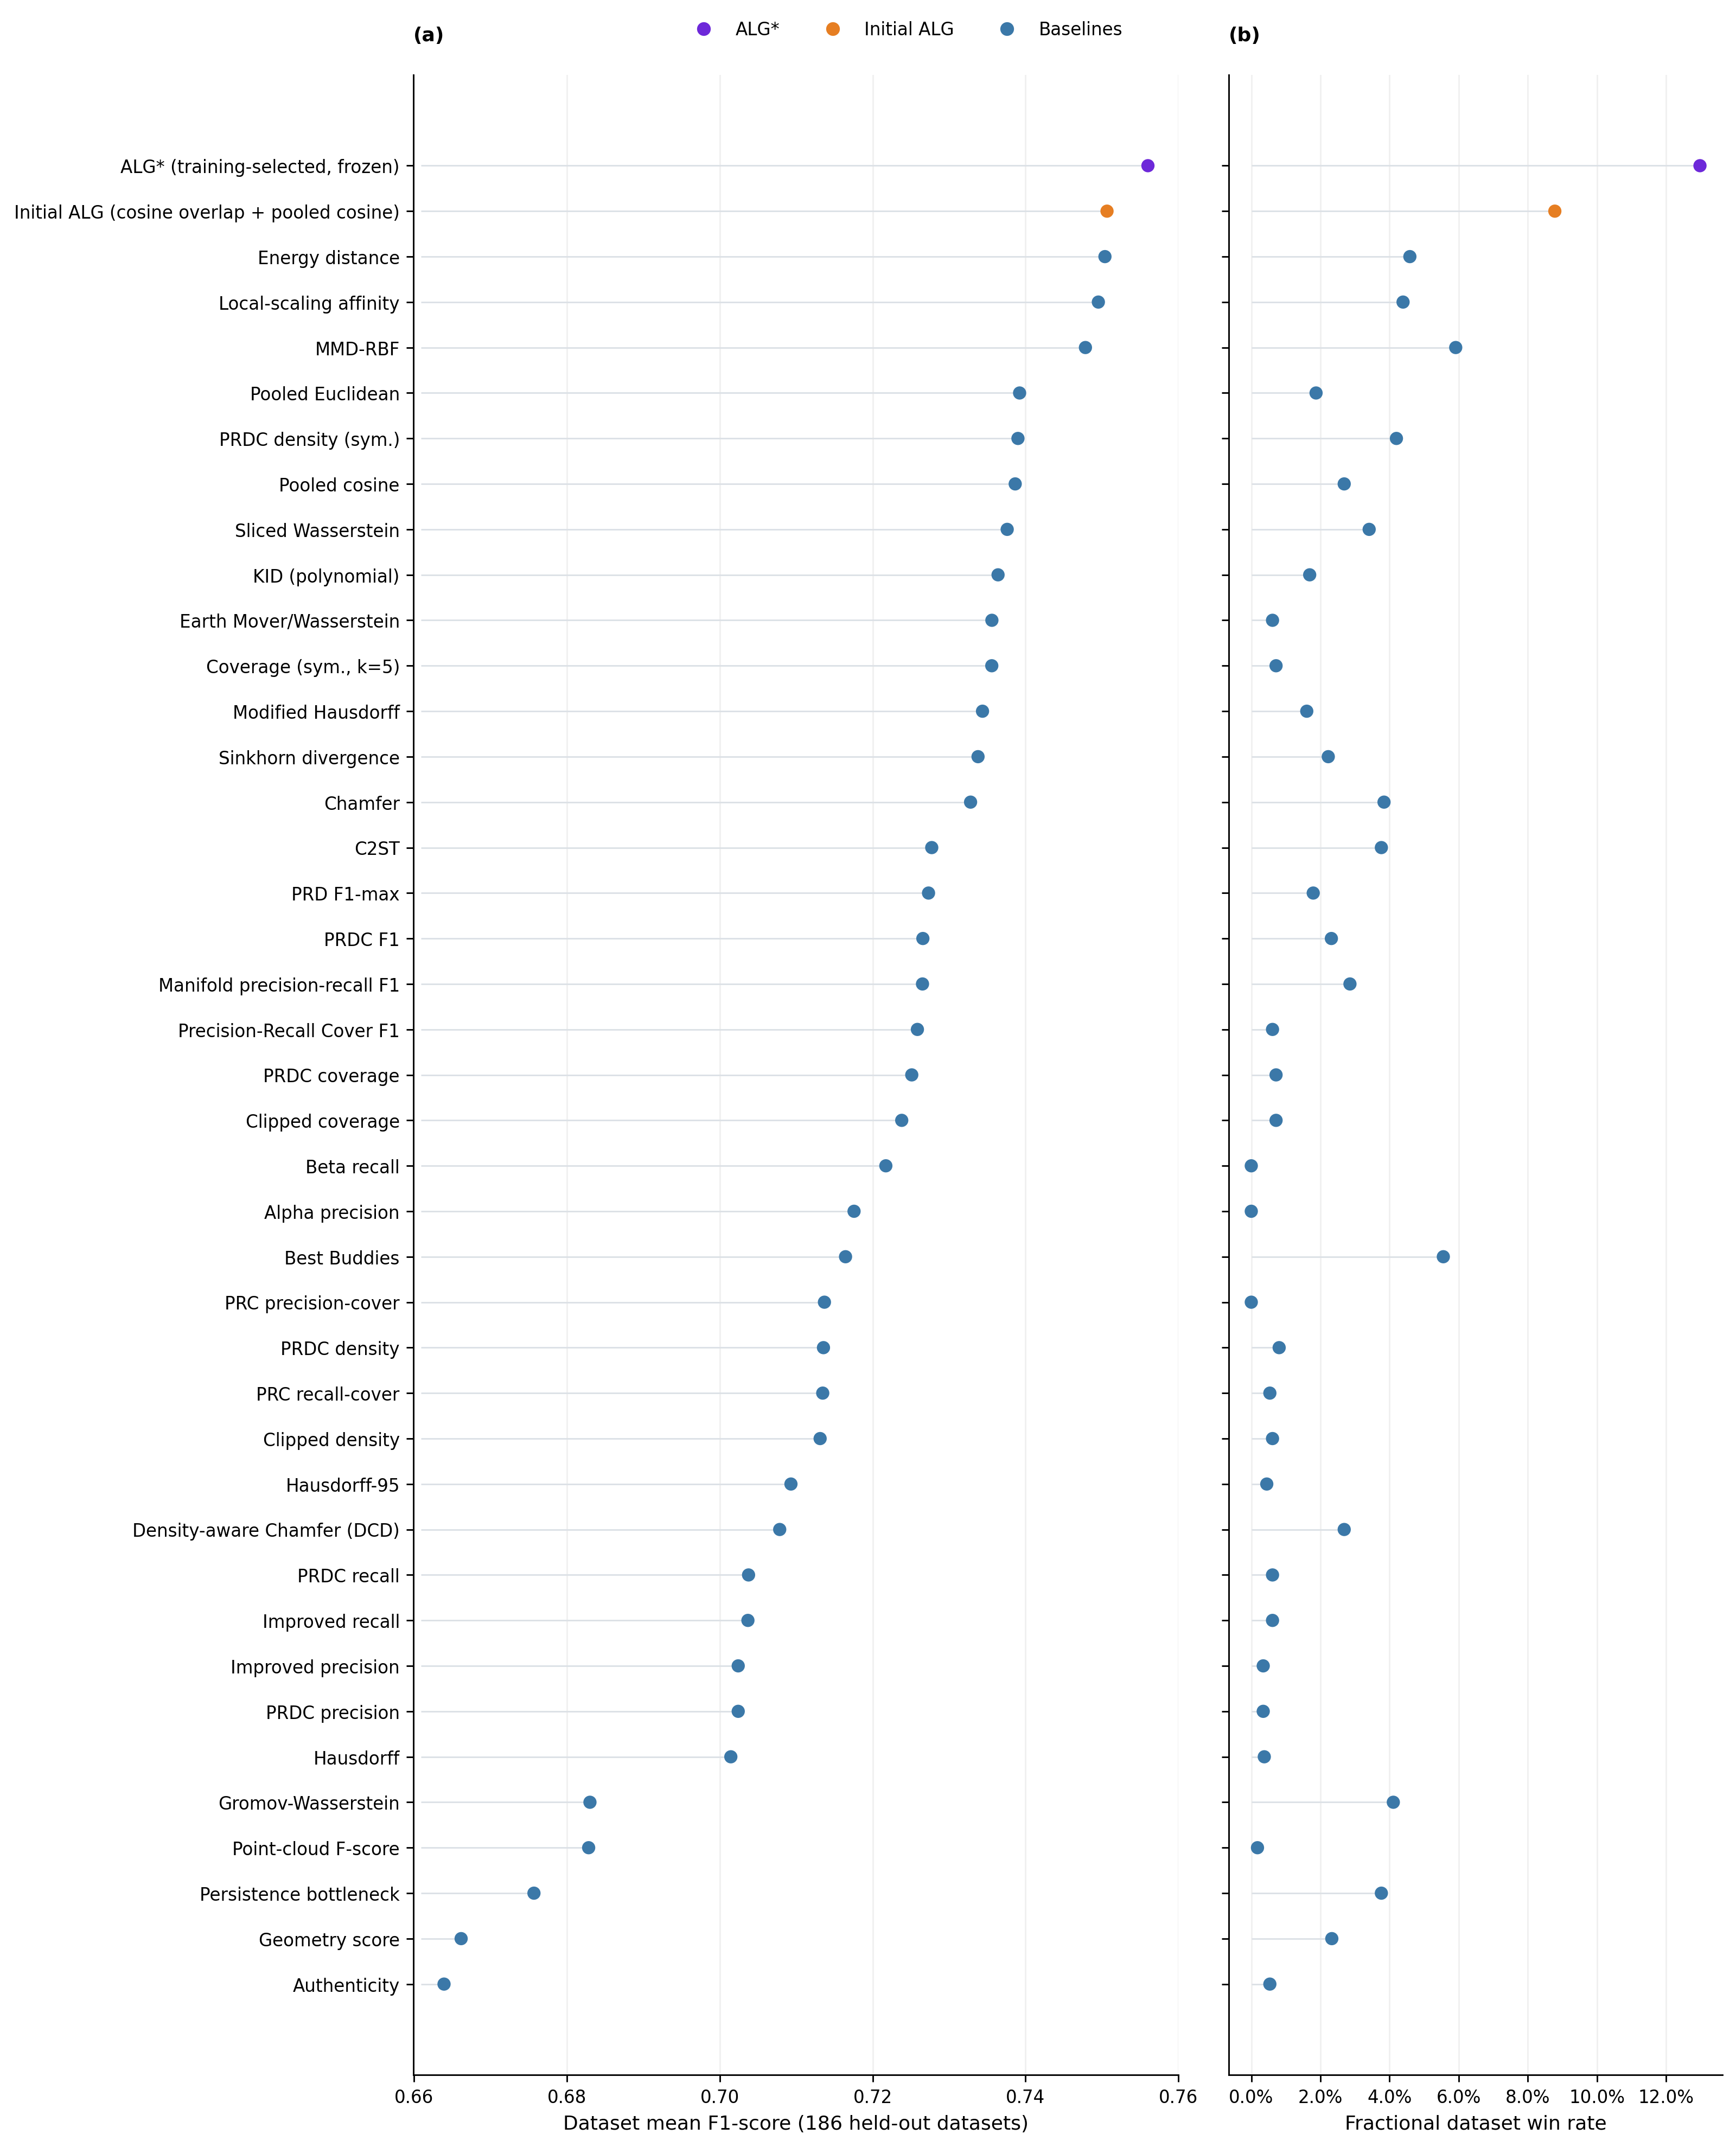
\includegraphics[width=\textwidth]{figures/01_confirmatory_leaderboard.png}
\caption{Mean positive-label F1-score and fractional dataset win rate
across 186 evaluation datasets. ALG$^*$ remains fixed from the
60 training datasets. This expanded overview is distinct from the
186-dataset confirmatory results in Table~\ref{tab:main}.}
\label{fig:leaderboard}
\end{figure*}

The paired comparison gives the same ordering. Against Energy distance,
ALG$^*$ has a mean paired F1-score difference of 0.0058, with a 95\% bootstrap
confidence interval of [0.0013, 0.0104]. ALG$^*$ is higher on 116 datasets and
lower on 67. The Holm-corrected Wilcoxon $p$-value is 0.0013. Initial ALG differs
from Energy distance by 0.0010 on average, with a bootstrap interval that
includes zero. This distinction is important: the stronger statistical result
is associated with the configuration selected on the training datasets, not
with the initial formulation alone.

\begin{table}[!htbp]
\centering
\caption{Paired comparison with Energy distance, the strongest external
baseline with complete test coverage. Holm correction is computed over all 40
baseline comparisons separately for each ALG method. The best value is bold;
the second-best value is underlined.}
\label{tab:paired}
\small
\begin{tabular}{lrrrr}
\toprule
ALG method & $\Delta$F1 & 95\% CI & W/T/L & Holm $p$\\
\midrule
ALG$^*$ & \textbf{0.0058} & [0.0013, 0.0104] & 116/0/67 & \textbf{0.0013}\\
Initial ALG & \underline{0.0010} & [-0.0047, 0.0065] & 96/7/80 & \underline{0.2431}\\
\bottomrule
\end{tabular}
\end{table}

\begin{figure*}[!htbp]
\centering
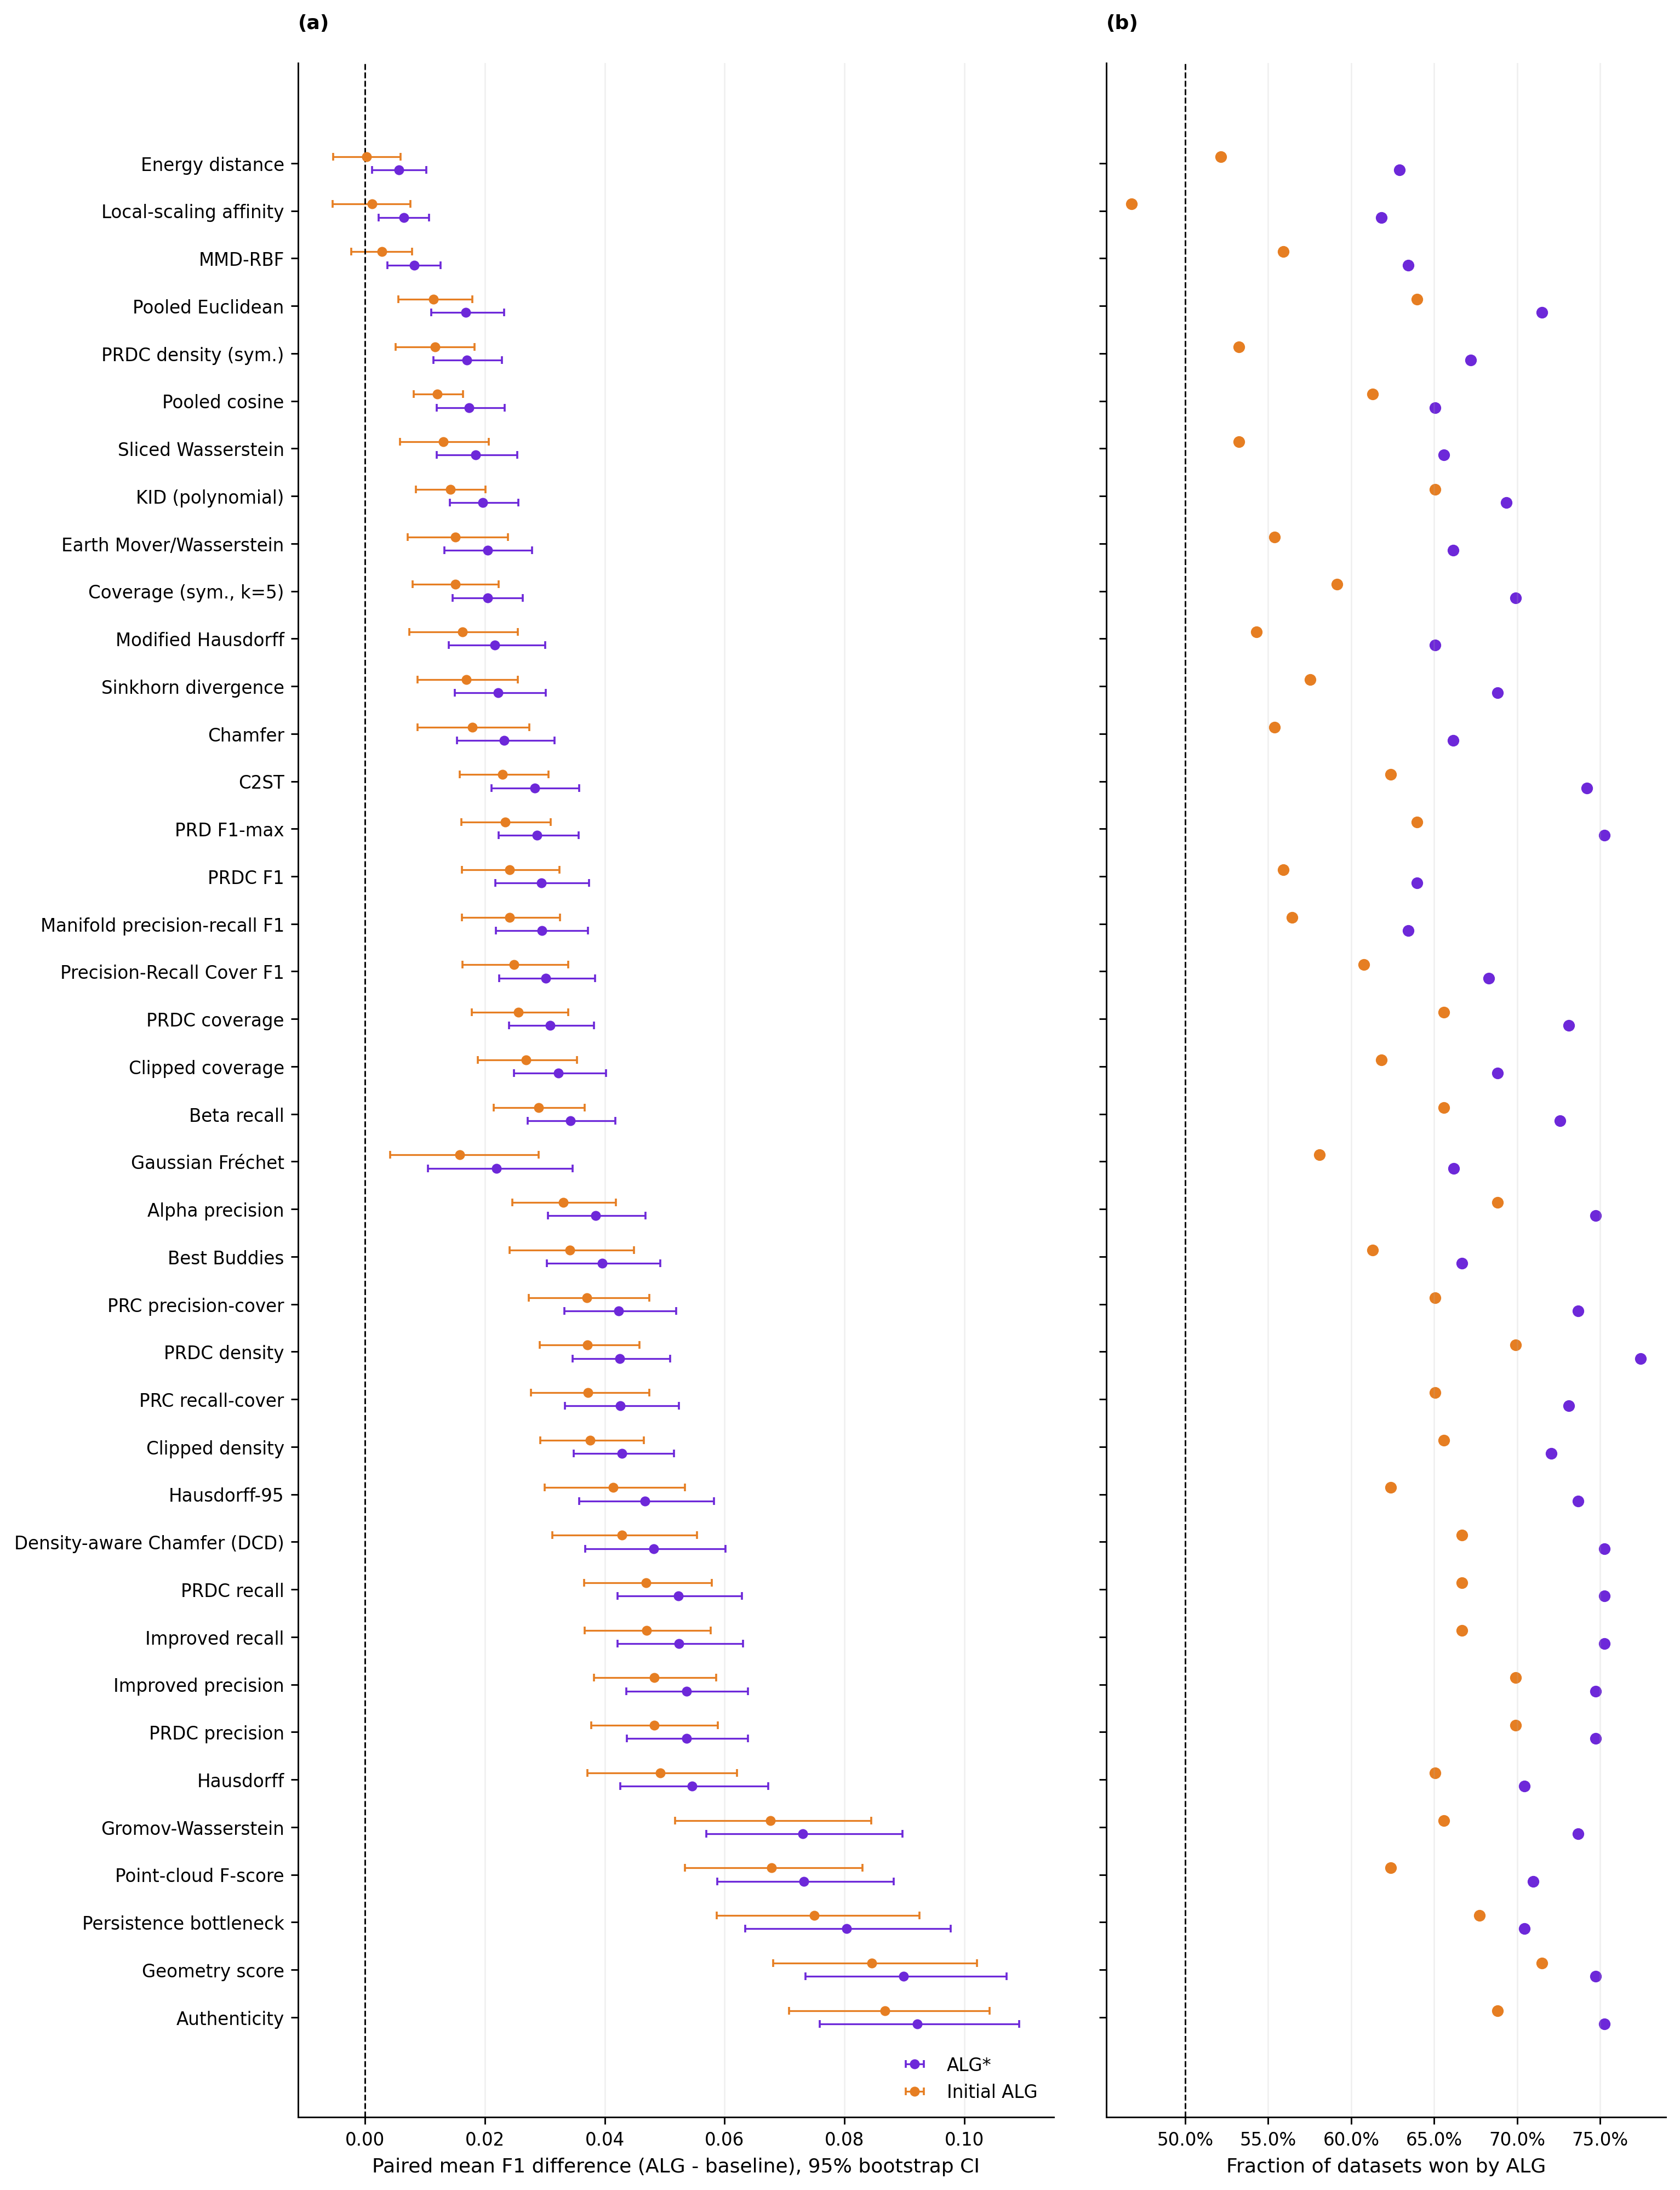
\includegraphics[height=0.80\textheight,keepaspectratio]{figures/05_paired_effects.png}
\caption{Paired F1-score differences and dataset win rates against all 40
baseline measures. Gaussian Fr\'echet is evaluated on the 133 test datasets for
which it is available; all other comparisons use 186 test datasets.}
\label{fig:paired}
\end{figure*}

The same fixed ALG$^*$ configuration is then examined by dataset family; no
family-specific configuration is selected. Figure~\ref{fig:category} retains
every comparison method so that variation between methodological families is
visible rather than restricted to a hand-picked subset. Table~\ref{tab:family}
reports the two ALG methods for reference.

ALG$^*$ reaches mean positive-label F1-score 0.6661 on graphs, 0.6684 on
images, 0.8738 on
OpenML, 0.9980 on the single tabular dataset, 0.7228 on text, and 0.7078 on time
series. The variation across families is substantial, and the selected ALG
configuration is not the highest-scoring method in every family. The relevant
observation is that the same selected configuration remains close to the
leading values across dataset families without test-time re-selection.

\begin{table}[!htbp]
\centering
\caption{The two ALG methods across the held-out dataset families. The complete
method-by-family comparison is shown in Figure~\ref{fig:category}. The best
value in each row is bold; the second-best value is underlined.}
\label{tab:family}
\small
\begin{tabular}{lrrr}
\toprule
Dataset family & $n$ & ALG$^*$ & Initial ALG\\
\midrule
Graphs & 15 & \textbf{0.6661} & \underline{0.6653}\\
Images & 12 & \textbf{0.6684} & \underline{0.6663}\\
OpenML & 57 & \textbf{0.8738} & \underline{0.8676}\\
Tabular & 1 & \underline{0.9980} & \textbf{0.9990}\\
Text & 6 & \underline{0.7228} & \textbf{0.7357}\\
Time series & 92 & \textbf{0.7078} & \underline{0.7016}\\
\bottomrule
\end{tabular}
\end{table}

\begin{figure*}[!htbp]
\centering
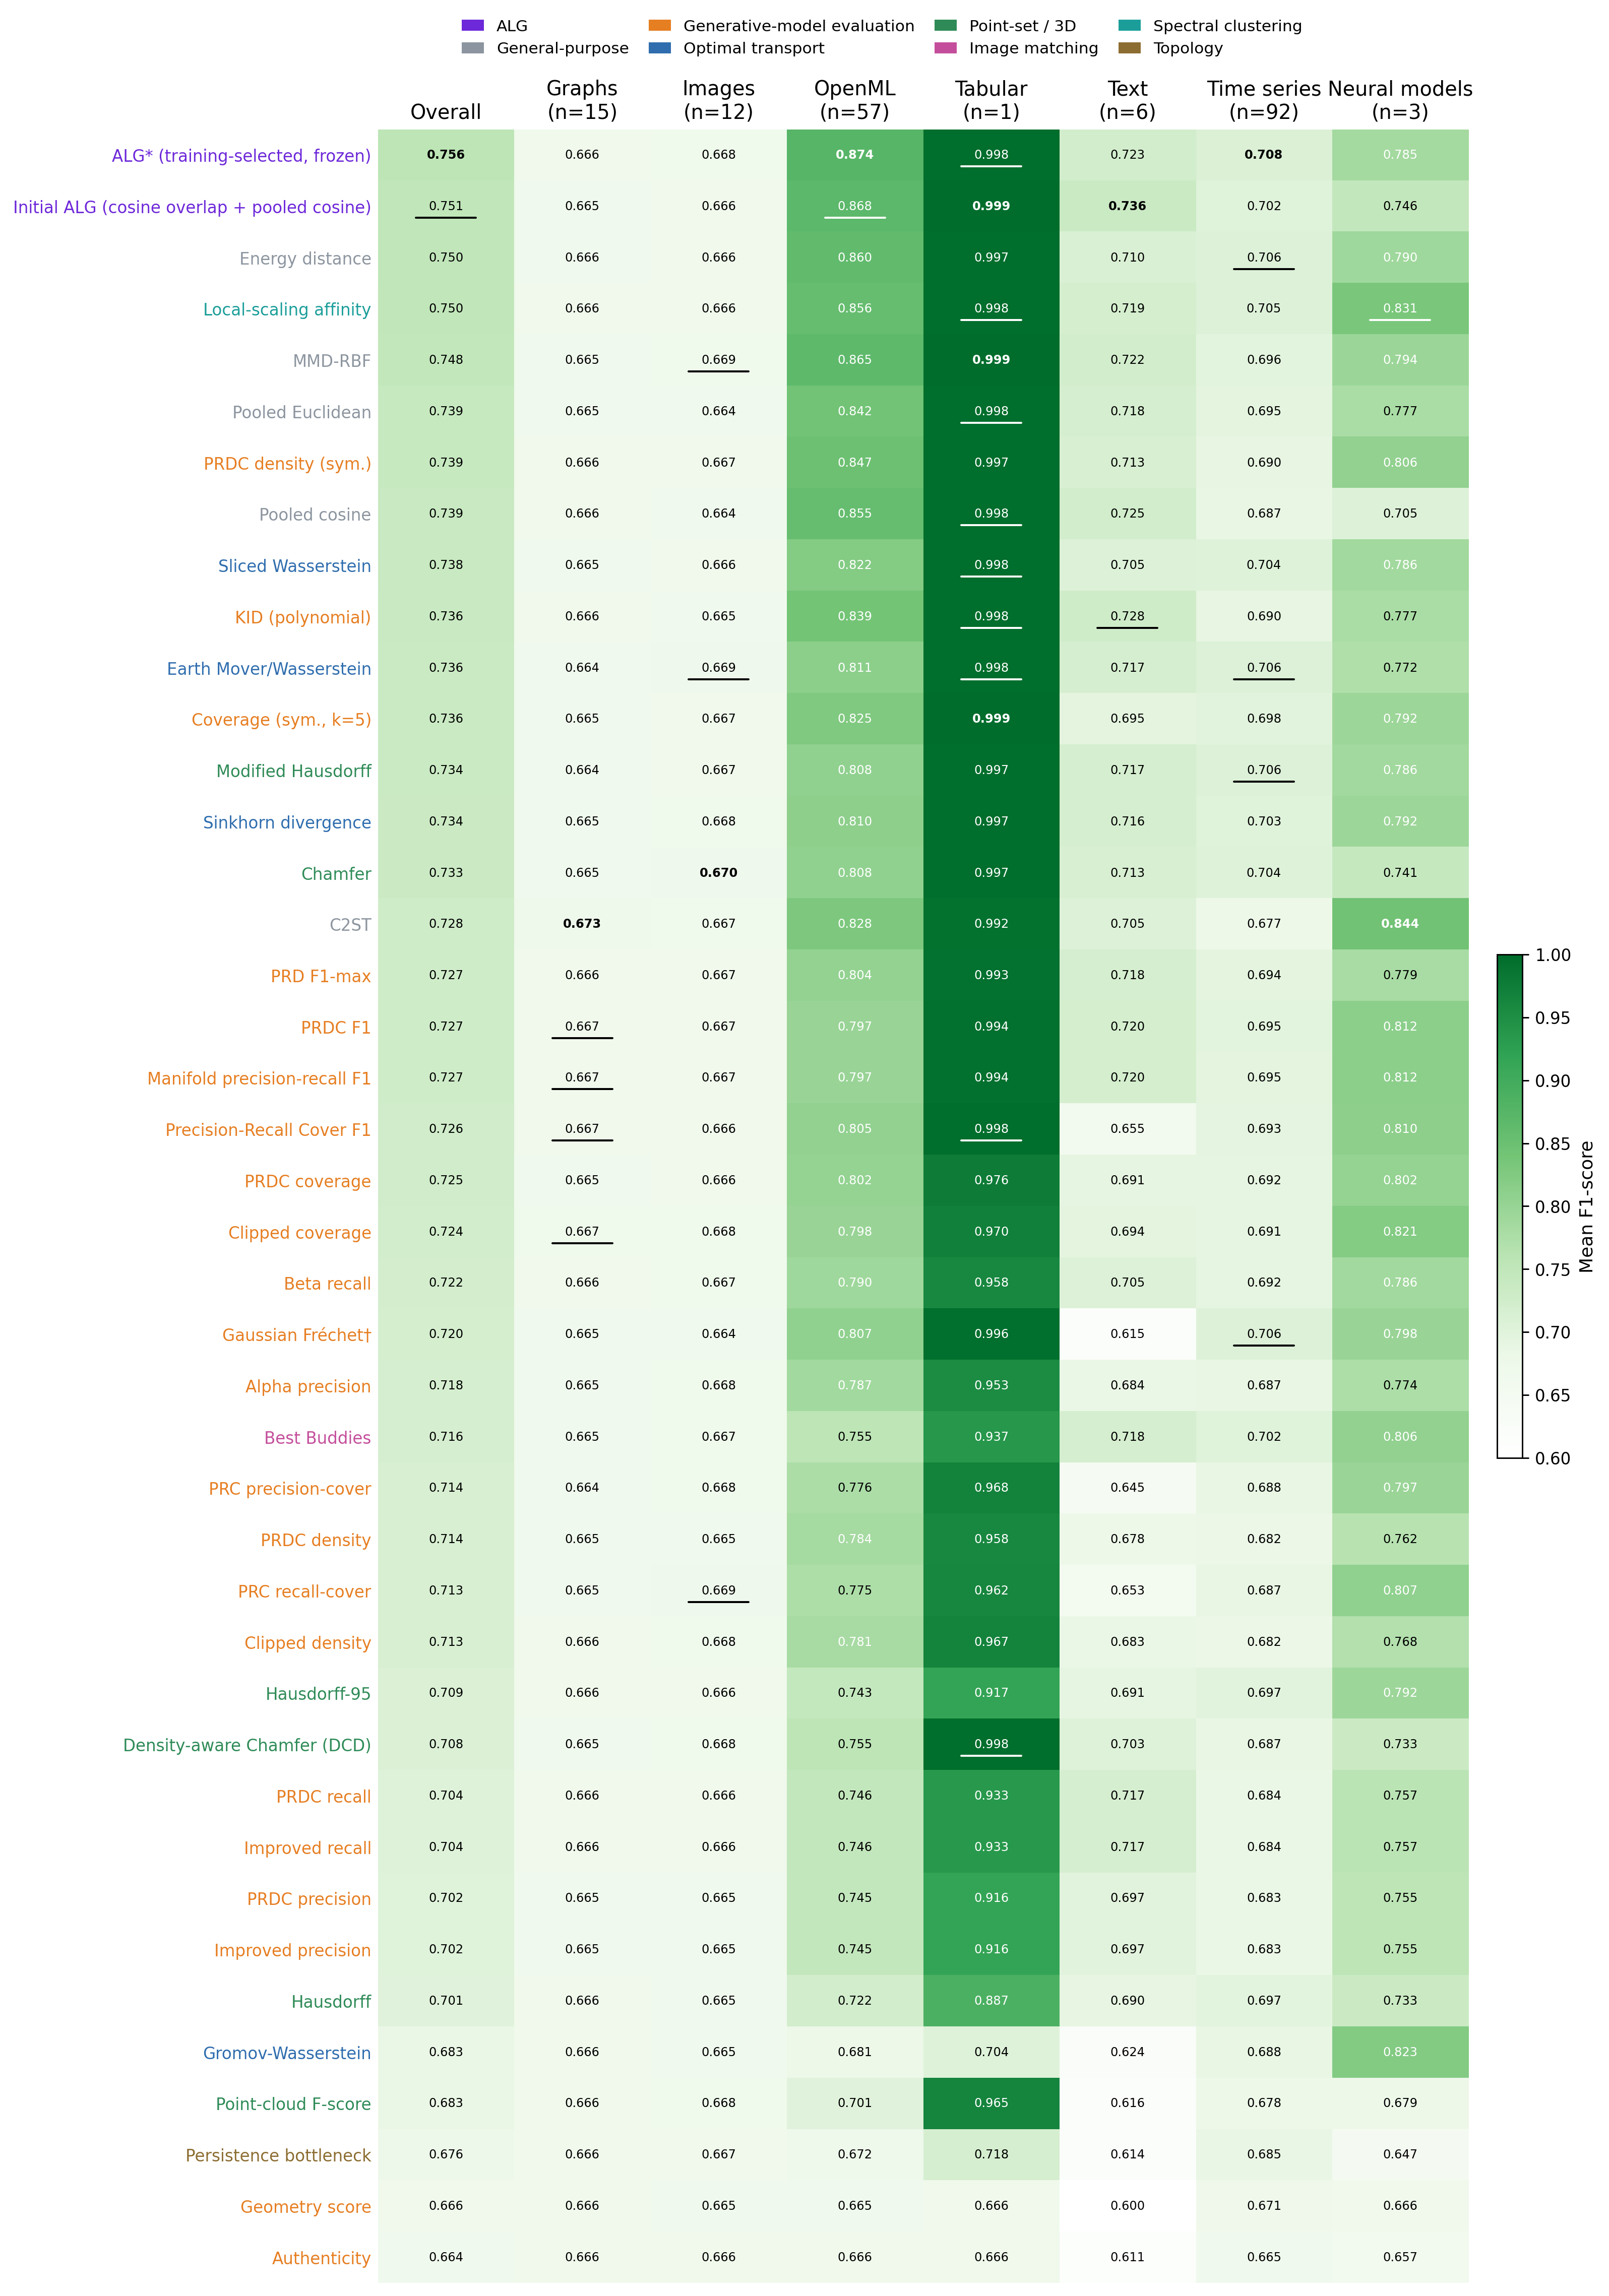
\includegraphics[height=0.80\textheight,keepaspectratio]{figures/03_category_performance.png}
\caption{Mean positive-label F1-score by dataset family for all comparison
methods. Graphs, images, OpenML, tabular data, text, and time series cover
186 held-out benchmark datasets; the neural-model column reports the three
additional datasets. The Overall column of this figure includes all
186 datasets and therefore differs from the 186-dataset estimates in
Table~\ref{tab:main}. The heatmap encodes F1-score, and colored method
labels indicate the original application domain; gray denotes general-purpose
methods. Gaussian Fr\'echet is available on 133 of the 186 held-out
benchmark datasets; its displayed means use available datasets only.}
\label{fig:category}
\end{figure*}

% \begin{figure*}[!htbp]
% \centering
% \includegraphics[height=0.82\textheight,keepaspectratio]{figures/09_neural_all_methods.png}
% \caption{Positive-label F1-score of all 46 available methods on the MNIST,
% KMNIST, and USPS
% neural-model-activation datasets. The final column reports the mean over the
% three datasets. Cell values are rounded to three decimals; column maxima are
% bold and the second distinct values are underlined. ALG$^*$ remains fixed from
% the 60 training datasets. The two internal rank-overlap variants in the
% 48-method taxonomy are unavailable for this protocol, leaving 46 methods.}
% \label{fig:neural}
% \end{figure*}
The three neural-model-activation datasets provide a separate
transfer check for the frozen configuration. ALG$^*$ reaches mean
positive-label F1-score 0.785 on these datasets, compared with 0.746 for
Initial ALG (values rounded from the additional evaluation). Other baselines
also achieve higher values on these representations; the complete comparison
is included in the neural-model column of Figure~\ref{fig:category}.

\FloatBarrier

% The three neural-model-activation datasets provide a separate transfer test for
% the frozen configuration. ALG$^*$ reaches mean positive-label F1-score 0.7847,
% compared with
% 0.7465 for Initial ALG. The best mean score is 0.8528 for symmetric overlap and
% overlap F1, followed by 0.8435 for C2ST. Thus, ALG$^*$ improves over Initial ALG
% on these representations but is not the best method in this small three-dataset
% evaluation. Figure~\ref{fig:neural} reports all 46 available methods without
% filtering by performance.

\paragraph{Discussion.}
The held-out comparison supports two distinct conclusions. First, Initial ALG
reaches a mean positive-label F1-score of 0.7507, compared with 0.7498 for
Energy distance,
0.7392 for Pooled cosine, and 0.7386 for Pooled Euclidean. However, its paired
difference from Energy distance is small and its confidence interval includes
zero. Second, configuration selection on the training datasets increases the
mean positive-label F1-score to 0.7556. The paired difference between ALG$^*$
and Energy
distance is positive under both the bootstrap analysis and the Holm-corrected
Wilcoxon test.

The magnitude of the improvement remains small and should not be interpreted
as universal dominance over every baseline or dataset. Different methods lead
on different dataset families, and the neural-model-activation evaluation also
shows that ALG$^*$ is not uniformly best. The evidence supports the more
specific conclusion that one training-selected local-global configuration
transfers across heterogeneous held-out datasets and improves the
mean positive-label F1-score across datasets over the strongest
complete-coverage external
baseline.

\FloatBarrier

\subsection{RQ2: Ablation}

Table~\ref{tab:ablation} compares each ALG method with its corresponding
local-only and global-only similarity on the same 186 held-out test datasets.
For Initial ALG, the local-only term is symmetric cosine overlap with $k=1$ and
the global-only term is exactly the Pooled cosine baseline of
Eq.~\eqref{eq:pooled-baselines}. The global-only Initial ALG value therefore
appears both in the baseline comparison and in this ablation by design; it is
the same similarity measure and the same result. For ALG$^*$, the local-only
similarity is local scaling with Manhattan distance and $k=3$, while the
global-only similarity is the normalized cosine-centroid component of
Eq.~\eqref{eq:selected-alg}.

\begin{table}[!htbp]
\centering
\caption{Matched local-only and global-only ablation. Wins/ties/losses compare
each component with the corresponding local-global ALG similarity. Within each
ALG block, the best score is bold and the second-best score is underlined.}
\label{tab:ablation}
\small
\begin{tabularx}{\linewidth}{lXrrr}
\toprule
ALG method & Variant & Mean $F1_{y=1}$ & Median $F1_{y=1}$ & W/T/L\\
\midrule
Initial ALG & Sym. cosine overlap ($k=1$) & \underline{0.7453} & \textbf{0.6887} & 81/9/93\\
Initial ALG & Pooled cosine & 0.7392 & 0.6698 & 53/19/111\\
Initial ALG & Local-global & \textbf{0.7507} & \underline{0.6813} & -\\
\midrule
ALG$^*$ & Local scaling ($L_1$, $k=3$) & \underline{0.7504} & \textbf{0.6874} & 63/19/101\\
ALG$^*$ & Normalized cosine centroid & 0.7391 & 0.6689 & 56/11/116\\
ALG$^*$ & Local-global & \textbf{0.7556} & \underline{0.6871} & -\\
\bottomrule
\end{tabularx}
\end{table}

The ablation shows that the local similarity obtains the higher mean
positive-label F1-score of the two individual similarities for each ALG method.
However, the local-global combination improves the mean positive-label
F1-score across datasets over the local similarity alone. This result is consistent with the
configuration frequencies in Figure~\ref{fig:prevalence}, where intermediate
values of $\lambda$ dominate the high-performing region.

\paragraph{Discussion.}
The matched ablation identifies the local similarity as the stronger individual
component of both ALG instances. Nevertheless, the local-global combination
obtains the highest mean positive-label F1-score in each block. The global similarity retains discriminative information on its own and
contributes complementary information when combined with the local similarity. The gain is modest, so the ablation
supports complementarity rather than claiming that fusion is superior on every
individual dataset.

\FloatBarrier

\subsection{RQ3: Configuration Stability}

The configuration space contains 168,960 alternatives, so the stability of
configuration selection must be evaluated explicitly. When all configurations
are ranked retrospectively on the 186 held-out test datasets, the configuration
selected on training ranks 196th, corresponding to the top 0.116\% of the
configuration space. The retrospective test optimum reaches mean
positive-label F1-score
0.7582, only 0.0026 above the selected score of 0.7556. The Spearman correlation
between training and test mean-positive-F1 rankings is $\rho=0.900$.

The training optimum is also part of a broad near-optimal region. The
difference between the first and second training configurations is
$1.535\times10^{-5}$. Three configurations are within 0.0001 of the training
maximum, 55 are within 0.001, 2,422 are within 0.005, and 25,701 are within
0.01. Figure~\ref{fig:devtest} shows the training-test association in the expanded
186-dataset evaluation and the size of the training near-optimal region. The result supports the stability of a
family of high-performing local-global configurations rather than the
uniqueness of one hyperparameter tuple.

\begin{figure*}[!htbp]
\centering
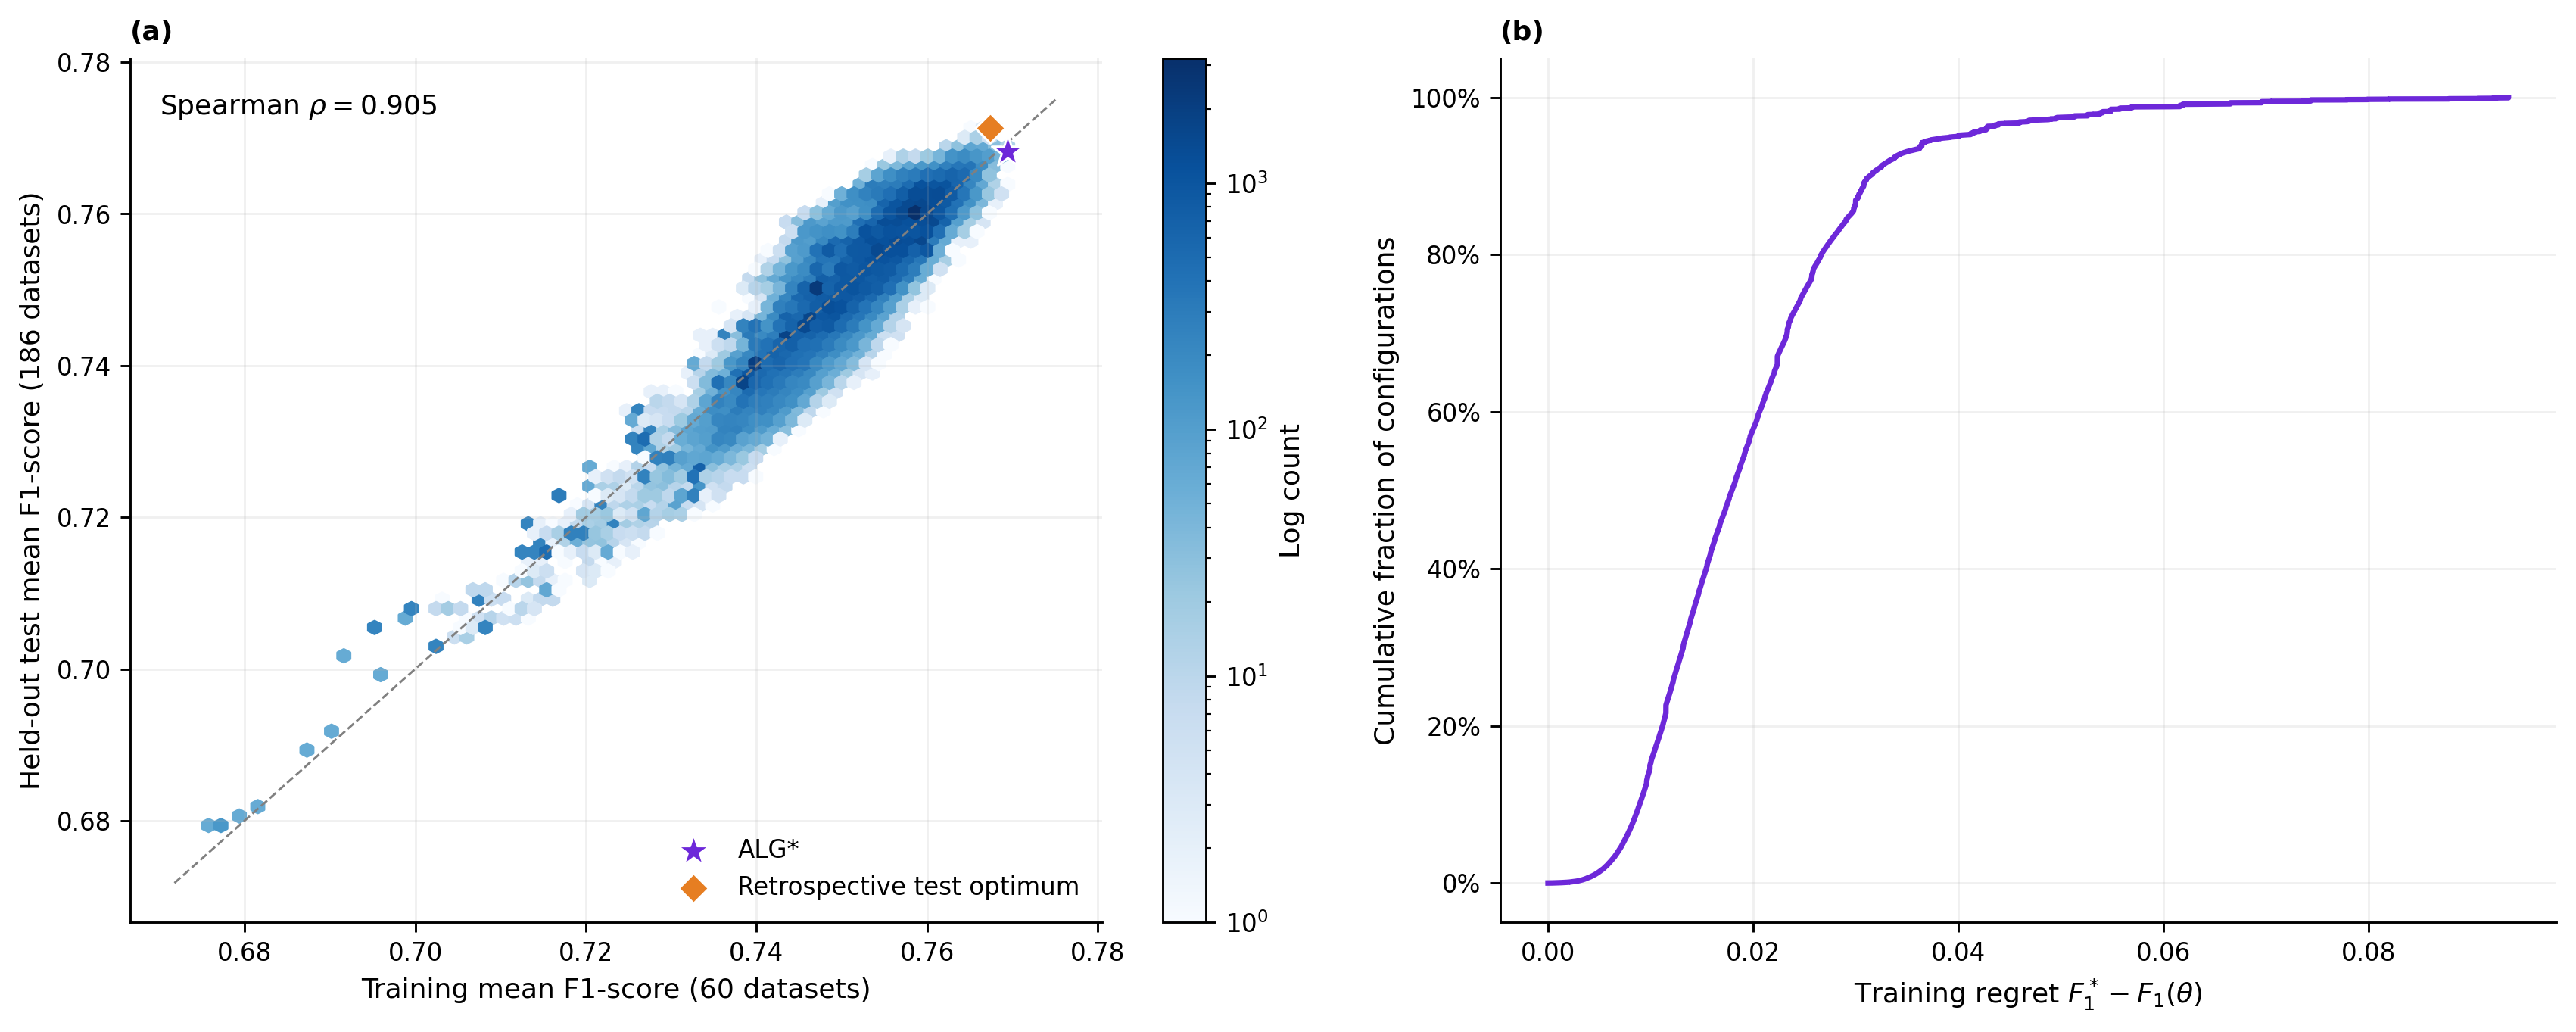
\includegraphics[width=0.96\textwidth]{figures/02_development_test_generalization.png}
\caption{Configuration-selection diagnostics over 168,960 ALG
configurations. Panel (a) plots the 60-training-dataset means against the
expanded 186-dataset evaluation means; Spearman $\rho=0.905$).
Panel (b) shows the cumulative proportion of configurations within a given
training regret. The 186-dataset analysis reported in the text is a separate
evaluation population.}
\label{fig:devtest}
\end{figure*}

The high-performing region also provides information about the selected design.
Among the top 1,000 training configurations, local scaling is used in 91.9\%
of the local similarities. Among configurations whose local similarity has a
neighborhood parameter, $k=3$ is used in 76.9\%. Manhattan, cosine, and
Euclidean geometries all remain represented. Centroid and Energy discrepancies
account for 48.1\% and 41.1\% of the global similarities, respectively, while
MMD accounts for 10.8\%. The local-global weights are concentrated between 0.3 and
0.8, so the high-performing region does not collapse to a local-only or
global-only similarity.

\begin{figure*}[!htbp]
\centering
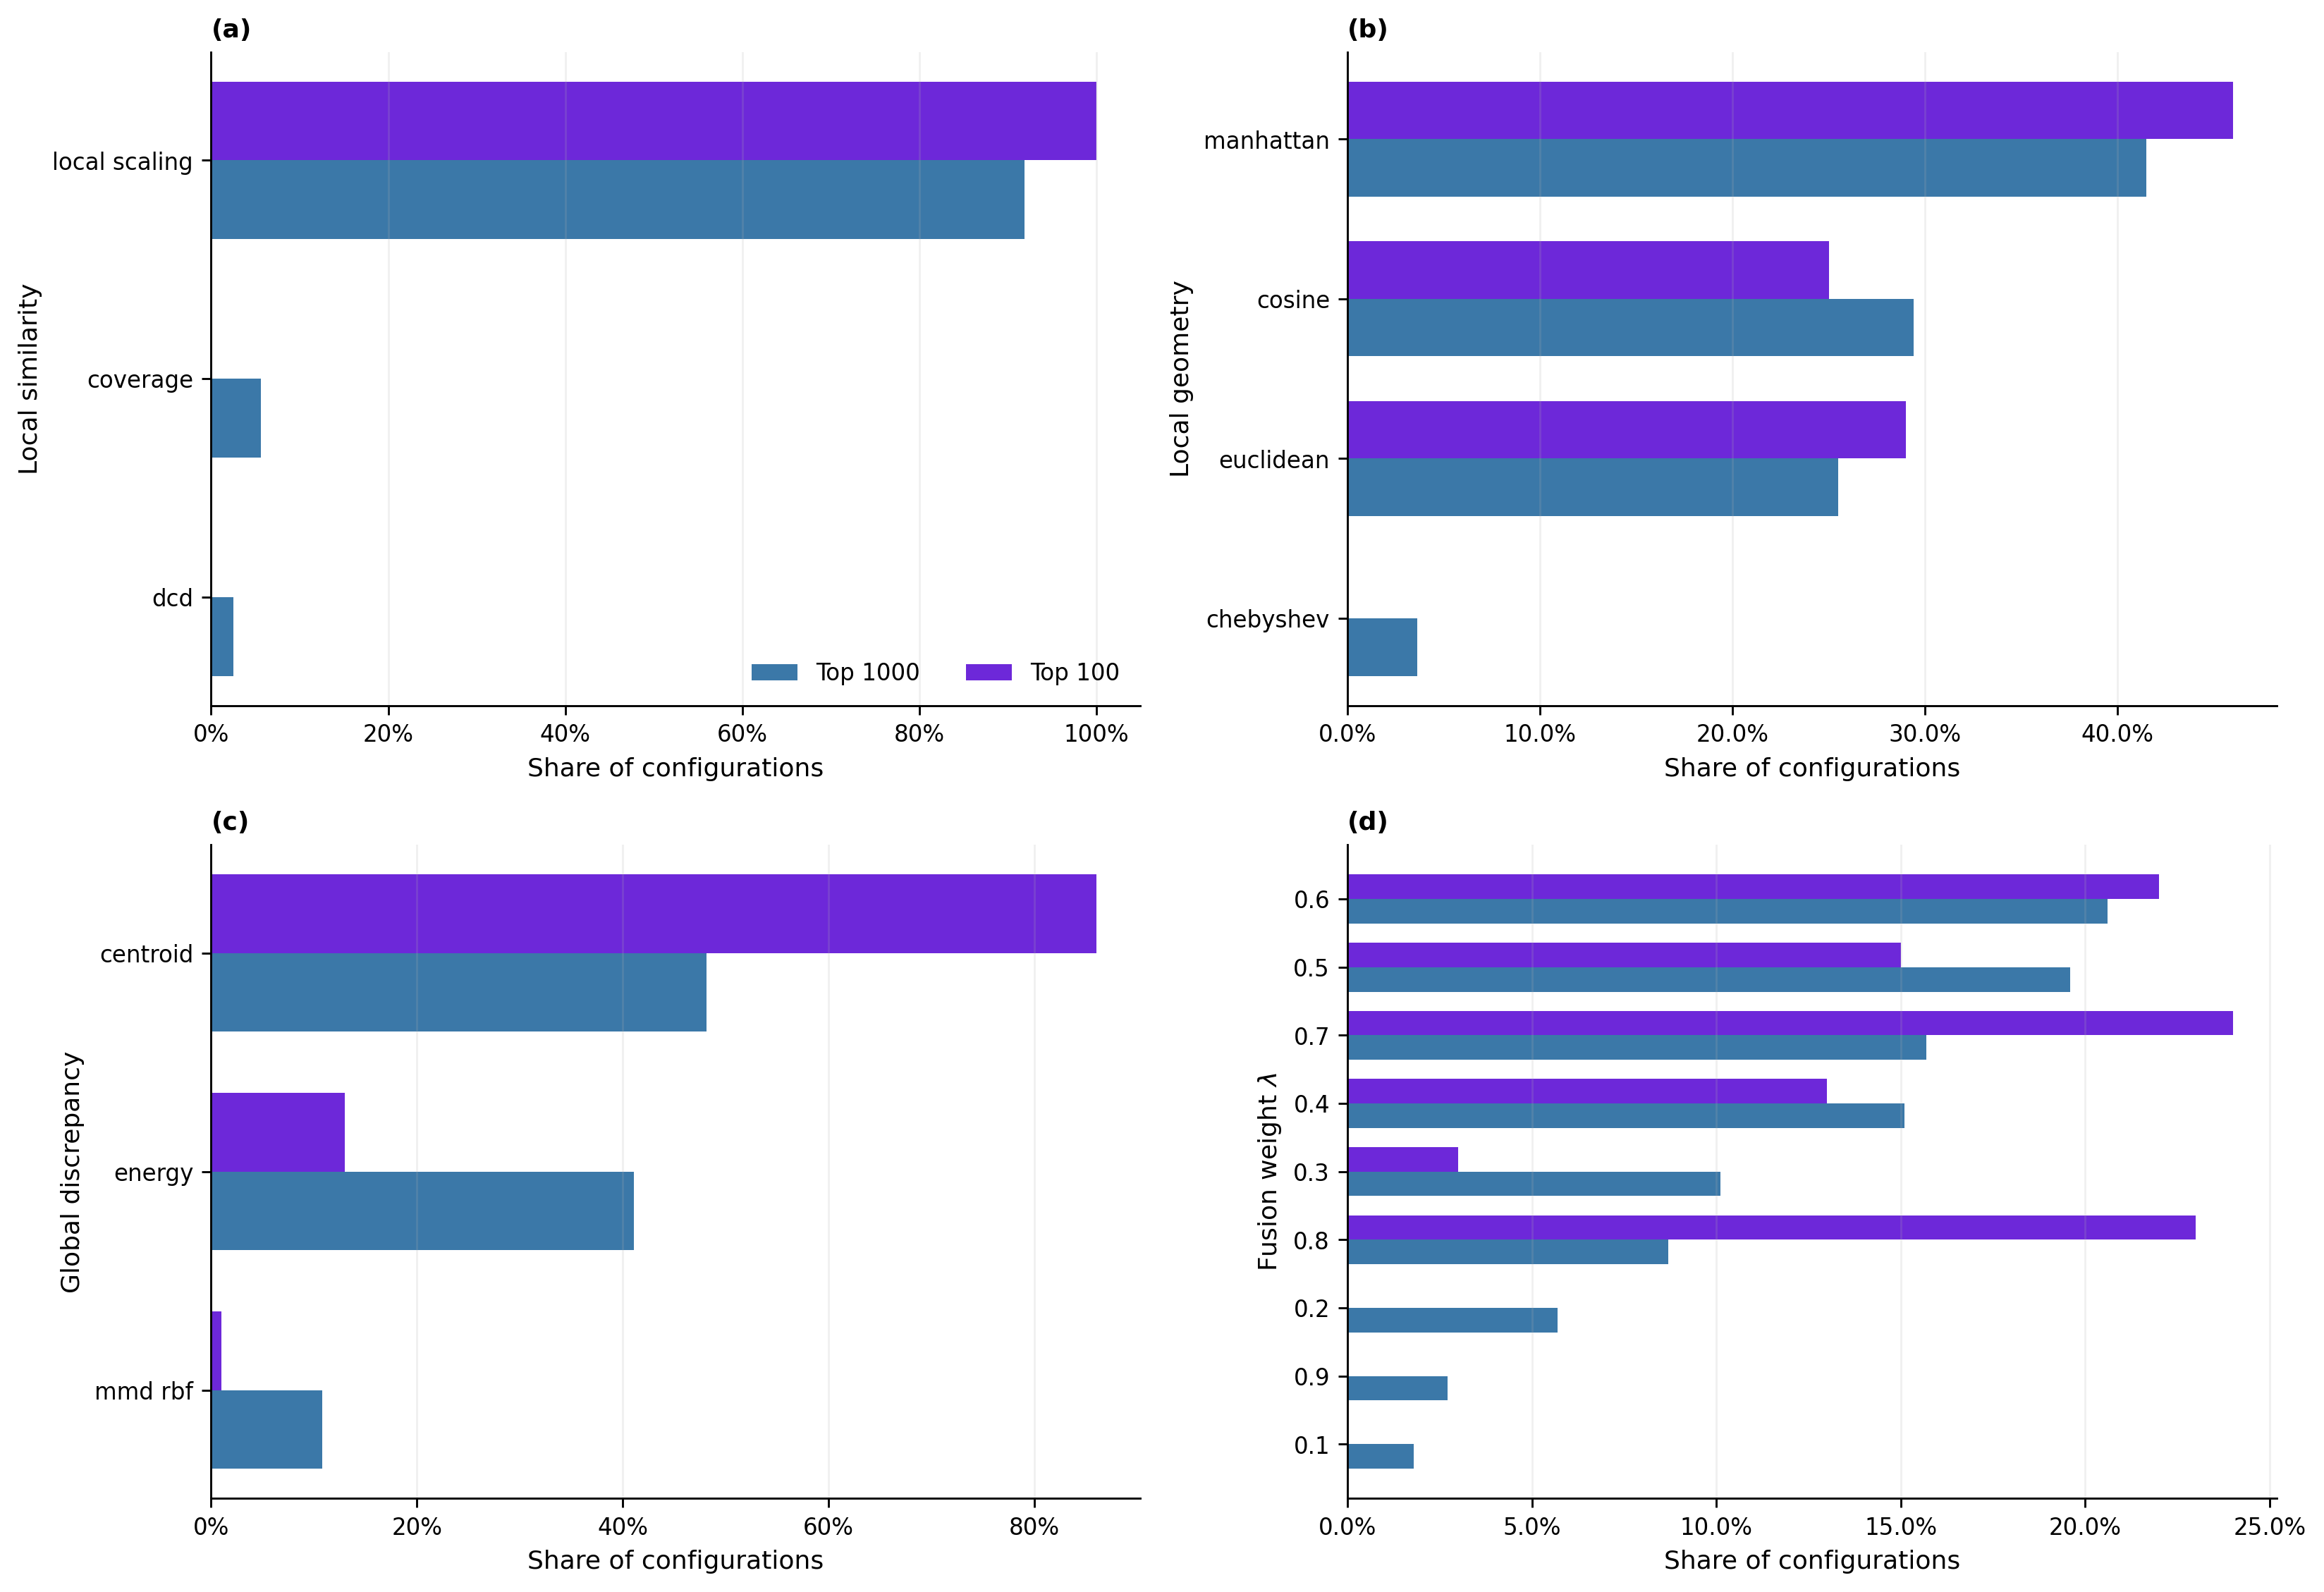
\includegraphics[width=0.96\textwidth]{figures/04_hyperparameter_prevalence.png}
\caption{Configuration frequencies among the top 100 and top 1,000 training
configurations. Intermediate local-global weights and local scaling are common
throughout the high-performing region.}
\label{fig:prevalence}
\end{figure*}

\paragraph{Discussion.}
A search over 168,960 configurations creates a risk of selecting an isolated
training optimum. The held-out analysis does not show this pattern: the
selected configuration ranks 196th retrospectively, the test optimum is only
0.0026 higher in mean positive-label F1-score, the training/test rank correlation is
$\rho=0.900$, and thousands of configurations lie close to the training
optimum.

These results do not establish that Manhattan distance, $k=3$, exponential
normalization, or $\lambda=0.7$ are universally optimal. They show that
configuration selection identifies a broad high-performing region in which an
adaptive local similarity is generally combined with a non-zero global
similarity.

\FloatBarrier

\subsection{RQ4: Sensitivity}

The controlled perturbation experiments characterize the response of the
similarity measures when the distributional difference is known.
Figure~\ref{fig:controlled} reports Gaussian translation, nested-support
scaling, and non-convex ring perturbations. It compares the frozen ALG$^*$
configuration with representative baselines. Each curve is min--max normalized
within method and panel; consequently, the figure compares response shape
rather than raw similarity values.

All three horizontal axes are oriented so that perturbation severity increases
from left to right. ALG$^*$ decreases monotonically across the three displayed
experiments. These experiments do not establish that one response shape is
universally preferable; they show how the selected local and global geometries
determine the changes to which ALG$^*$ is sensitive.

\begin{figure}[!htbp]
\centering
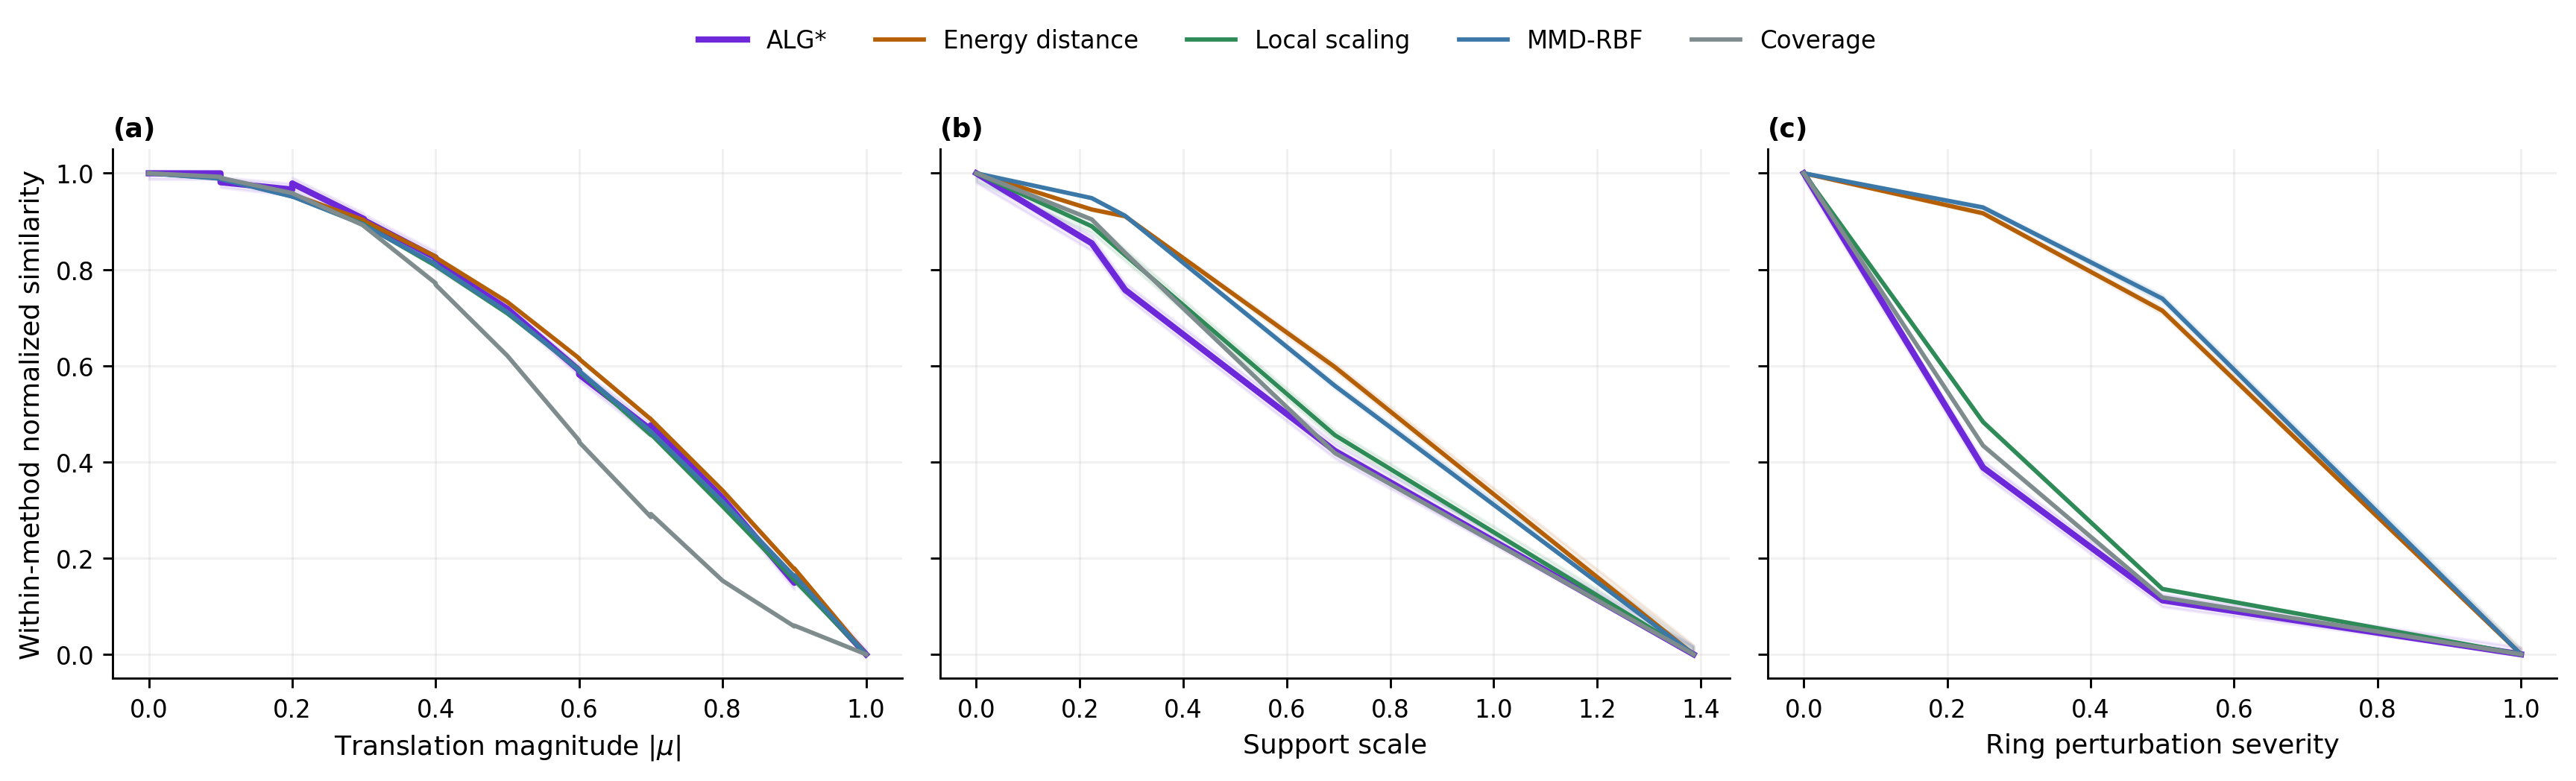
\includegraphics[width=0.96\textwidth]{figures/07_controlled_perturbations.png}
\caption{Controlled perturbation response of ALG$^*$ and representative
baseline measures. The horizontal axes are oriented so that perturbation
severity increases from left to right. Similarities are min--max normalized
within each method and panel.}
\label{fig:controlled}
\end{figure}

Figure~\ref{fig:controlled-all} complements the response curves with an
exhaustive comparison of ALG$^*$ and all 40 baselines. For each method and
perturbation, the cell reports the negative Spearman correlation between
perturbation severity and mean similarity. A value near one denotes a monotone
decrease in similarity, a value near zero denotes a weak monotone response,
and a negative value denotes the opposite orientation. For nested support,
severity is the absolute log-ratio from equal support. This matrix summarizes
sensitivity rather than discriminative F1-score and does not identify one
response profile as universally preferable.

\begin{figure*}[!htbp]
\centering
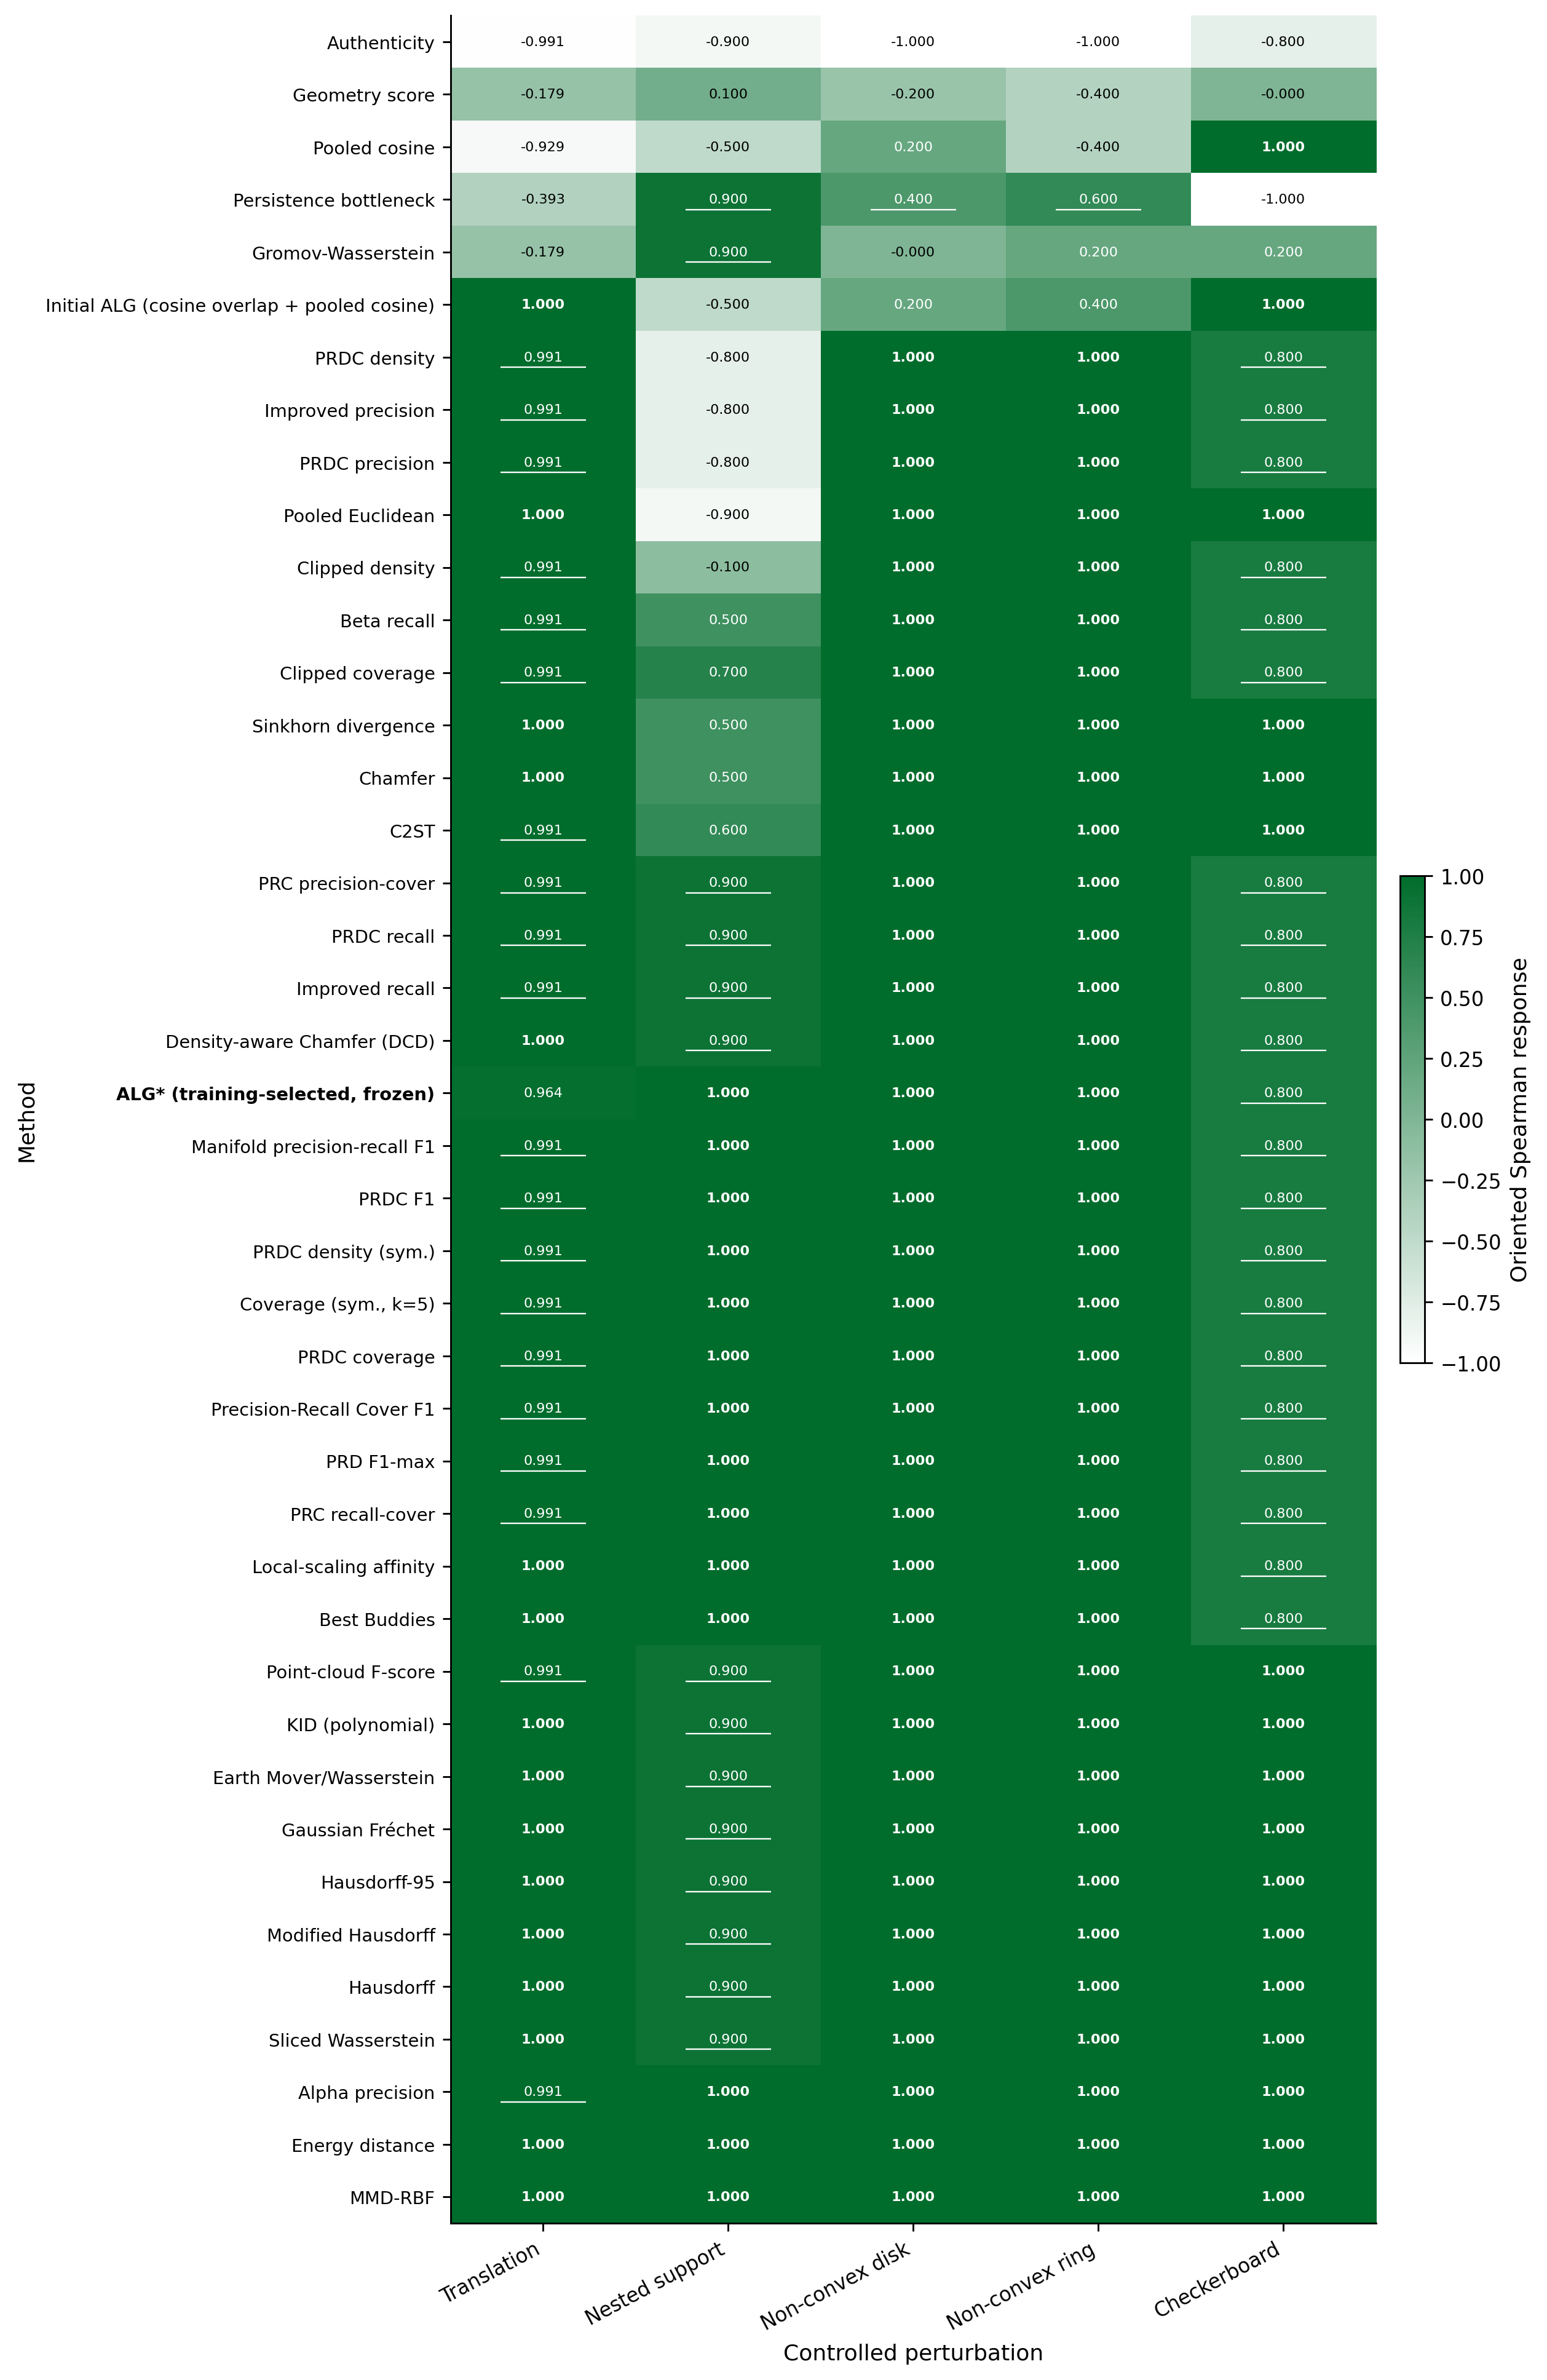
\includegraphics[height=0.88\textheight,keepaspectratio]{figures/08_controlled_all_baselines.png}
\caption{Controlled sensitivity of ALG$^*$ and all 40 baselines across five
multi-level perturbations. Cells show the oriented Spearman response computed
from the mean similarity at each perturbation level.}
\label{fig:controlled-all}
\end{figure*}

\paragraph{Discussion.}
The controlled experiments show that ALG$^*$ responds monotonically to the
displayed perturbations. Its response is determined jointly by its adaptive
local-scaling component and its normalized global cosine-centroid component.
The comparison also confirms that different baseline families respond to
different perturbation geometries. These results characterize the sensitivity
profile of the frozen ALG$^*$ configuration rather than establishing universal
superiority under every controlled perturbation.
\subsection{RQ5: Efficiency}

To answer RQ5, we measure both deployment-time efficiency and the one-time
cost of configuration selection. Deployment-time measurements are performed
on the same 155,393 embedding-set pairs from the 183 test datasets. For
ALG$^*$ and Initial ALG, each similarity is recomputed end-to-end from the raw
embedding sets without reusing cached distances or framework components. Each
method is executed independently three times per pair, and the median elapsed
time is retained before aggregation.

ALG$^*$ requires an average of 0.780 ms per embedding-set pair, compared with
1.046 ms for Initial ALG. The selected configuration therefore reduces the
end-to-end runtime by 25.4\%, corresponding to a $1.34\times$ speedup over the
initial formulation. Figure~\ref{fig:runtime} reports these measurements
together with the recorded runtimes of all 40 baselines and the explicitly
labeled diagnostic computations. The diagnostic totals and ALG-family totals
are internal measurements and are not additional baselines.

\begin{figure*}[!htbp]
\centering
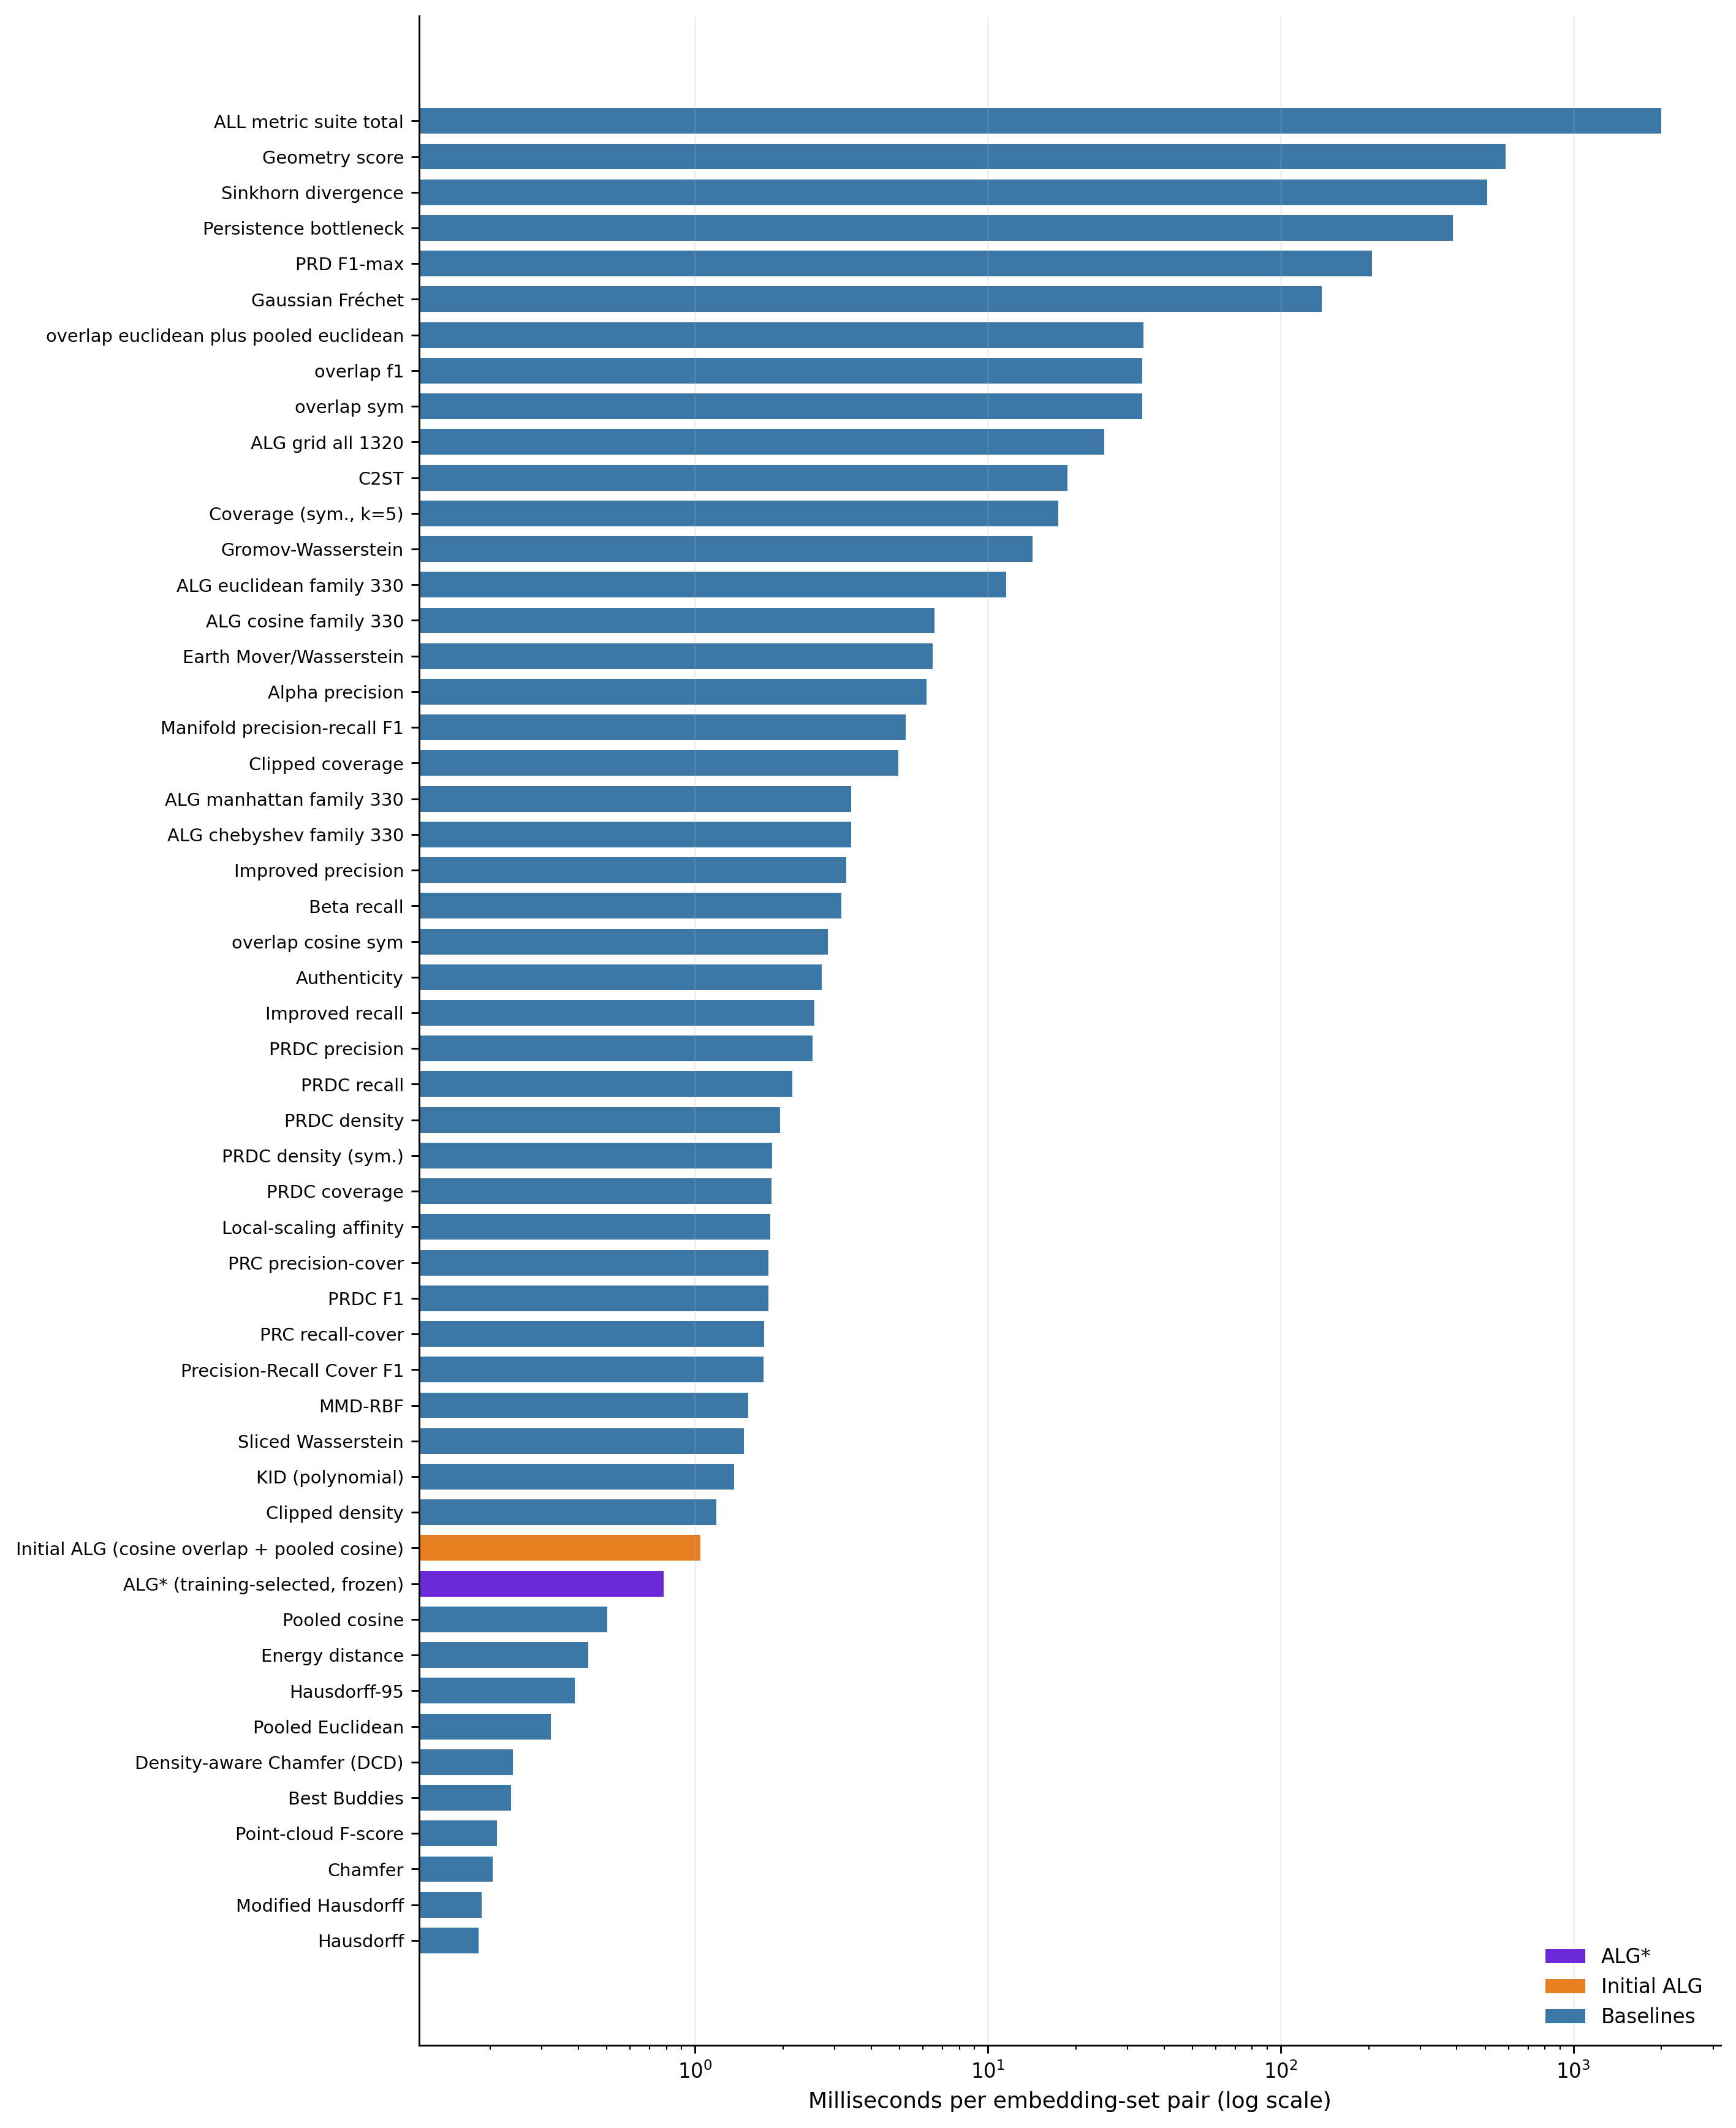
\includegraphics[width=0.92\textwidth]{figures/06_runtime_comparison.png}
\caption{Measured end-to-end runtime per embedding-set pair on 155,393 pairs
from the 183 test datasets. ALG$^*$ and Initial ALG are recomputed from the raw
embedding sets without cached components; their reported values aggregate the
median of three independent executions per pair. The figure also includes all
40 baselines and explicitly labeled diagnostic computations. Diagnostic totals
and ALG-family totals are not additional baselines. The horizontal axis uses a
logarithmic scale.}
\label{fig:runtime}
\end{figure*}

Among the 40 baselines, ALG$^*$ is faster than 30 and slower than 10. The
methods that remain faster are predominantly simple pooled or geometric
comparisons, whereas several distributional, optimal-transport, topological,
and classifier-based metrics require substantially more computation. Thus,
ALG$^*$ improves both effectiveness and runtime relative to Initial ALG, but it
is not the fastest method in absolute terms.

Across the 243 eligible datasets, cumulative component computation requires
7.39 task-hours and evaluation of the 168,960 scalar local-global combinations
requires 3.27 task-hours. These values are sums over parallel tasks rather than
Slurm wall-clock time. The median component-computation time is 8.68 s per
dataset and the median configuration-evaluation time is 54.27 s per dataset.

\paragraph{Discussion.}
The efficiency results distinguish the one-time cost of selecting ALG$^*$ from
its deployment-time cost. The exhaustive search is made feasible by computing
reusable local and global components during training. Once the configuration
is frozen, however, ALG$^*$ is evaluated directly and does not require the
complete component grid. Its measured runtime of 0.780 ms per pair shows that
the selected local--global formulation remains inexpensive at deployment and
is 25.4\% faster than Initial ALG. Nevertheless, simpler pooled and geometric
baselines can be faster, so the result establishes a favorable
effectiveness--efficiency trade-off rather than a universal runtime advantage.

\subsection{Limitations}

The test datasets are not balanced across dataset families. The held-out split
contains 92 time-series datasets and 57 OpenML datasets, but only six text
datasets and one tabular dataset. Dataset averaging prevents datasets with
many embedding-set pairs from dominating the result, but it does not give equal
weight to each dataset family. In addition, datasets from the same archive, such
as UCR or OpenML, can share construction characteristics; the 186 held-out
datasets should therefore not be interpreted as 186 independent application
domains.

Gaussian Fr\'echet is available on only 133 held-out test datasets. We report
its coverage explicitly and retain the strict 133-dataset common-subset comparison rather
than imputing missing values. The retrospective test optimum over the 168,960
ALG configurations is used only to analyze selection stability and must not be
interpreted as a confirmatory competitor. The runtime comparison also combines
component-based ALG timing with monolithic timing for most baseline measures,
so it is not a controlled systems benchmark.

Finally, the binary threshold is calibrated within each dataset. This protocol
isolates the ordering induced by the similarity measure, but it does not test
whether one universal decision threshold transfers across datasets. Applications
that require a fixed threshold need a separate calibration experiment. 


\section{Conclusion}
\label{sec:conclusion}

We define Adaptive Local-Global similarity (ALG) for the comparison of finite
unordered embedding sets. ALG combines an adaptive local similarity, whose
scale is estimated from within-set nearest neighbors, with a normalized global
similarity. The local similarity, global discrepancy, geometry, normalization,
and local-global weight remain explicit configuration choices.

The selected ALG configuration is chosen using 60 training datasets and is
then evaluated without further configuration selection on 186 held-out test
datasets. It reaches a mean positive-label F1-score across datasets of 0.7556,
compared with
0.7498 for Energy distance, the strongest literature baseline with complete test
coverage. The matched ablation shows that the local and global similarities
provide complementary information, and the controlled perturbation experiments
show that the response of ALG depends on the geometry encoded by its local and global similarities.

The main result is therefore not that one geometry is universally optimal.
Rather, a local-global similarity can be selected without test leakage and can
retain competitive performance across heterogeneous dataset families while
keeping its geometric assumptions explicit. This makes ALG applicable as a
similarity layer in information-system and machine-learning pipelines that
compare sets of learned representations.

% \section{Complete comparator suite and coverage}
% \label{app:comparators}

% Table~\ref{tab:all-comparators} reports the fixed method taxonomy used in the
% main analysis. It contains exactly two ALG methods, 38 literature baselines, and two
% standard pooled baselines. Six internal ALG components or alternative
% configurations are reserved for ablation and configuration analysis. Gaussian Fr\'echet is the
% only baseline with partial test coverage and is marked with a dagger.

% \input{tables/complete_comparator_suite.tex}

% To compare Gaussian Fr\'echet on the same test datasets as every other method,
% Figure~\ref{fig:common133} evaluates all 42 comparison methods on the strict
% 133-dataset common subset.

% \begin{figure*}[!htbp]
% \centering
% \includegraphics[width=0.84\textwidth]{figures/07_common133_all_methods.png}
% \caption{All 42 comparison methods on the strict 133-dataset common subset.
% This analysis includes Gaussian Fr\'echet without mixing unequal test
% coverage.}
% \label{fig:common133}
% \end{figure*}

% \section{Principal artifact files}
% \label{app:artifact}

% \begingroup
% \small
% \sloppy
% \begin{itemize}
% \item \path{framework_configurations_168960.csv}: configuration file for the completed 168,960-configuration campaign.
% \item \path{framework_development_ranking.csv}: dataset ranking used for configuration selection on the training datasets.
% \item \path{method_roles.csv}: fixed taxonomy distinguishing ALG methods, internal ALG components, literature baselines, and standard pooled baselines.
% \item \path{all_primary_methods_by_support.csv}: complete method-by-dataset-family matrix used in Figure~\ref{fig:category}.
% \item \path{paired_two_alg_vs_all_baselines.csv}: paired comparisons of Initial ALG and ALG$^*$ with all 40 baseline measures.
% \item \path{baseline_results_test186.csv.gz}: per-dataset results for the baseline measures.
% \item \path{f1_matrix_all243.npz}: complete ALG F1-score matrix over the 243 eligible datasets.
% \item \path{dataset_catalog_250.csv}: dataset provenance, construction rules, pair counts, partition, and exclusions.
% \item \path{ablation_initial_and_selected_test186.csv}: matched local-only and global-only ablation for Initial ALG and ALG$^*$.
% \item \path{all_scores.csv}: controlled perturbation results over 145 conditions and 128 random seeds.
% \item \path{SHA256SUMS}: integrity manifest for the reproducibility artifact.
% \end{itemize}
% \endgroup

\bibliographystyle{elsarticle-num}
\bibliography{references}

\end{document}
